\documentclass[]{article}

\usepackage{graphicx}
\usepackage{url}
\usepackage{amsmath}
\usepackage{amssymb}
\usepackage{amsthm}
\usepackage{hyperref}
%\usepackage[margin=1.5in]{geometry}
\usepackage{microtype}

\renewcommand{\familydefault}{phv}

%opening
\title{Data Management for Distributed Sensor Networks: A Literature Review}
\author{Anthony J. Christe}

\begin{document}

\maketitle


\begin{abstract}
    Sensor networks can benefit from the generally ``unlimited resources'' of the cloud, namely processing, storage, and network resources. This literature review surveys the major components of distributed data management, namely, cloud computing, distributed persistence models, and distributed analytics.
\end{abstract}

\pagebreak

\tableofcontents
\listoffigures
\pagebreak

\section{Introduction} \label{sec:introduction}
The exponential increase in volume, variety, velocity, veracity, and value of data has caused us to rethink traditional client-server architectures with respect to data acquisition, storage, analysis, quality of data, and governance of data. With the emergence of Internet of Things (IoT) and increasing numbers of ubiquitous mobile sensors such as mobile phones, distributed sensor networks are growing at an unprecedented pace and producing an unprecedented amount of streaming data. It's predicted by the European Commission that IoT devices will number between 50 to 100 billion devices by 2020\cite{6072197}.

The size of sensor networks is quickly growing. BBC Research provides figures that the market share for sensor networks in 2010 was \$56 billion and was predicted to be closer to \$91 billion by the end of 2016 \cite{zaslavsky_sensing_2013}. Data generated from the IoT are surpassing the compute and memory resources of existing IT infrastructures. \cite{chen_big_2014}. Not only is the size of data rapidly exploding, but data is also becoming more complex. Data from sensor networks is often semi-structured on unstructured with data quality issues. 

Sensor networks can benefit from the generally ``unlimited resources'' of the cloud, namely processing, storage, and network resources. We believe that by leveraging cloud computing, distributed persistence models, and distributed analytics, it's now possible to provide a platform that is able to meet the demands of the increasing distributed sensor market and the increasing volume, velocity, variety, and value of data that comes along with that. 

This review summarizes the current state of the art surrounding distributed sensor networks and the use of cloud computing as a means for big sensor data acquisition and analysis. In particular, we will define Big Data and review it in the context of sensor networks, review cloud computing and service models related to distributed sensing, discuss modern distributed persistence for Big Data, and modern distributed analytics for Big Data all with an emphasis on acquiring and managing Big Sensor Data.

\subsection{Applications of Distributed Sensor Networks} \label{ssec:applications-of-distributed-sensor-networks}
Zaslaveky et al. \cite{zaslavsky_sensing_2013} cites several examples of distributed sensor networks in-the-wild including: a real-time greenhouse gas detection network deployed across California, real-time structural monitoring such as the St. Anthony Falls Bridge sensor network in Minneapolis, distributed radiation detection in Fukushima, real-time parking space inventory in San Francisco.

Perera et al. in their paper on sensing as a service\cite{perera_sensing_2014} provide three examples of areas distributed sensor networks would accelerate at. 

First, distributed sensors could be used by cities to optimize waste management which consumes a significant amount of time, money, and labor. Waste management also has many processes including collection, transport, processing, disposal, and monitoring. By collecting and storing sensor data in the cloud from these processes, various interested parties could access sensor data in order to optimize for the current state of the system. As an example, Perera mentions that city council members could optimize garbage routes and collection rates based on the amount of trash available and recycling centers could forecast what to expect based off of the same sensor data. Basically interested parties at all points of the management process could benefit by analyzing data points from IoT devices in a smart city.

Second, Perera mentions that smart agriculture can take advantage of distributed sensor networks and cites the  \textit{Phenonet} project as an example of distributed agricultural sensing which has the ability to monitor plant growth, soil composition, air composition, and pests. A major advantage of this system is that it can supplement traditional research by allowing multiple researchers access to the same data in near real-time.

Third, Perera postulates that environmental management could utilize existing distributed environmental sensors upgraded to communicate with the cloud allowing for data sharing and data fusion among interested parties.

Gerla et al.\cite{gerla_internet_2014} propose an internet of vehicles as a means to autonomous vehicles. By treating vehicles as platforms of thousands of sensors each and by creating dynamic distributed clouds, they hope to allow fleets of vehicles to make autonomous decisions. This model uses distributed clouds based on proximity and peer-to-peer to technologies rather than sending data to a centralized cloud. The real-time nature and the size and amount of sensors makes this an interesting case study.

%% smart grid
One area that shows a lot of promise for distributed sensor networks with centralized management is smart grids. The smart grid is an collection of technologies aiming to advance the electrical grid into the future with respect to intelligent energy distribution and integration of renewable. Electrical grids can benefit by using a large distributed sensor network to collect power consumption, production, and quality information and use that information to control power production and consumption in real-time. 

In some cases, the sensor nodes in smart grids lack powerful local computation abilities, but generally have network connections and sensing capabilities. This makes the cloud a perfect sink of information for analyzing complex power trends from a large scale distributed sensor network for smart grids\cite{botta_integration_2016}.

\subsection{Rest of this Review} \label{ssec:rest-of-this-review}
The rest of this review is structured as follows: Section \ref{sec:big-sensor-data} provides an overview of Big Sensor Data\ref{sec:big-sensor-data}. Section \ref{sec:cloud-computing} will focus on cloud computing and how its concepts can be utilized to manage distributed sensor data. Section \ref{sec:big-data-persistence-models} will examine the current state of the art distributed persistence models with an emphasis on how NoSQL and distributed persistence models can aid in managing distributed sensor data. Section \ref{sec:big-data-analytics} will examine the current state of big data analytics options in the cloud and how these can be utilized for performing analytics on distributed sensor data.

\section{Big Data} \label{sec:big-sensor-data}
Big Data is described using many definitions. Cox, in 1997\cite{cox_managing_1997}, provides us with one of the earliest definitions where Big Data is ``too large to be processed by standard algorithms and software on the hardware one has available to them''. He also mentions that sources for big data collections include data from remote sensors and satellite imaging in the fields of atmospheric sciences, geophysics, and healthcare.

Cox separates Big Data into big data into two categories; namely, \textit{big data collections} and \textit{big data objects}. 

Big data objects are single, very large data sets such as computational models computed from physical phenomena. Big data objects often do not fit in memory or local disks. Big data objects also have adverse affects on bandwidth and latency. Cox looks to moving computation to the data and more advanced segmentation and paging techniques at the OS level to deal with big data objects.

Big data collections contain many smaller objects or even many big objects. Big data collections present their own set of issues including: distributed data, heterogeneous data formats, no platform independent definition, non-local meta-data, large storage requirements, poor locality, and insufficient network resources. 

Cox provides us a useful definition to build on. He also advocates for the development and advancement of operating system constructs for moving data that is too large for memory in and out of memory using stenciling, segmentation, paging, and application controlled segmentation. It's interesting to note that this was before cloud computing and distributed systems, but we are now facing similar problems at the distributed level rather than a local level.

The Apache Hadoop project, in 2010, defined big data as ``datasets which could not be captured, managed, and processed by general computers within an acceptable scope''\cite{chen_big_2014}.

Manyika et al\cite{manyika} in 2011 define big data as ``the amount of data just beyond technology's capability to store, manage, and process efficiently'' essentially making the definition of big data a moving target that is constantly evolving as technology becomes updated.

The Whitehouse report on big data\cite{pcast}, in 2014, defines big data as "data that is so large in volume, so diverse in variety or moving with such velocity,that traditional modes of data capture and  analysis  are  insufficient" and 

Hashem et al.\cite{hashem_rise_2015} build on these previous definition in their 2015 review on Big Data providing the definition by attempting to create a definition that encompasses the spirit of many of the previous definitions. They define big data as ``a set of techniques and technologies that require new forms of integration to uncover large hidden values from large datasets that are diverse, complex, and of a massive scale''.

NIST, in 2015, \cite{nist_big_data_2015} provide multiple definitions relating to big data. NIST defines big data as ``extensive datasets--primarily in the characteristics of volume, variety, velocuty, and/or variability--that require a scalable architecture for efficient storage, manipulation, and analyst. To my knowledge, NIST is the only organization to specify the need of a scalable architecture alongside its definition of big data. NIST next defines the big data paradigm as ``the distribution of data systems across horizontally coupled, independent resources to achieve the scalability needed for the efficient processing of extensive datasets''.

Perhaps one of the most popular definitions of Big Data is characterizing data by ``the four Vs''\cite{hashem_rise_2015}, \textit{volume}, \textit{variety}, \textit{velocity}, and more recently, \textit{value}. 

\subsection{The Three (Four and Five) ``V's"}
The first mention of the three V's was in Laney's 2001 article \textit{3-d data management: controlling data volume, velocity, and variety}\cite{laney20013d}. Laney describes the challenges of managing e-commerce data by categorizing the data challenges into three dimensions. First, we will review Laney's definition of the 3 V's and then we will examine updated, expanded, and more modern interpretations of the three V's and also look at the more recent ``fourth V''.

Volume is the amount of data flowing into a system at any one time. Laney argues that the increased availability of the internet to anyone as an e-commerce platform greatly increases the amount of transactional data stored on server backends. Since data is a tangible asset, organizations may be reluctant to discard the data. At the same time, as the amount of data increases, each individual data point becomes less important. Laney mentions that if organizations are not willing to simply buy more online storage, that they can take the following steps to limit volume growth: implement tiered storage systems, limit data collected to only data required for current organization processes, limit analytics to statistically sampled data, eliminate redundancy in data sources, offload ``cold spots'' to cheaper storage (i.e. tape), and outsorce data management. 

In terms of the increase in data volume, we can look at several statistics starting from the year 2011 and working onwards. According to Gantz et al.\cite{gantz_extracting_2011}, the world wide accumulation of data in 2011  was around 1.8 zettabytes. Then in 2013, during the D11 conference, Meeker presented that this figure had risen to 5 zettabytes across the globe. In 2014, more than 500 million photos were uploaded every day and more than 200 hours of video per minute\cite{pcast}. Tweets generate 12 terabytes of data per day\cite{sharma_extended_2015}.  Perera et al.\cite{perera_sensing_2014} expect with IoT, we could see as many as 1 billion sensors online and generating data by the year 2020. Power meters generate upwards of 350 billion readings annually\cite{sharma_extended_2015}. According to IBM\cite{ibm}, ``90\% of the world's data has been created in the past two years''. 

Velocity is defined by Laney as ``increased point-of-interaction (POI) speed and, consequently, the pace data used to support interactions and generated by interactions'', or more generally, the pace of data arriving and how long it takes to analyze, store, and act on that data. Laney offers several solutions to data velocity in using operational data stored that prioritizes production data, front-end caching, point-to-point data routing protocols, and architecting software in such a way that balances data analysis latency with stated real-time requirements. Some examples of high velocity data include GPS tracking data, web site click streams, social media interactions, and data from mobile sensors\cite{pcast}. Sharma et al.\cite{sharma_extended_2015} also mention that over 5 million trade transactions must be processed daily for fraud detection. 

Laney describes data variety as data that is in ``incompatible formats, non-aligned data structures, and inconsistent data semantics''. Laney's proposed solutions to variety include profiling data to find inconsistencies, a standardized XML data format, interprocess application communication, middlewares on top of ``dumb data'' to provide meaning and intelligent, metadata management, and more advanced indexing techniques. The main reason for the increase in variety of data is due to the prevalence of internet connected devices and the internet of things (IoT) explosion. We now see a wide variety of data that was \textit{born analog} such as sensors measuring our physical world like temperature, solar radiance, power quality, seismic activity, acoustics, etc. We also see much more variety in \textit{born digital data} from the web, social media, government databases, geospatial data, surveys, healthcare, etc\cite{pcast}.

Value is often added as a fourth "V" and represents the value that can only be gained by finding insights into big data. Manika et al. in their McKinsey report\cite{manyika2011big} describe the value of big data after studying the results of long running big data healthcare projects. Value in terms of efficiency and quality of data can be gained from big data using cross correlations and data fusion to gain insights that was not possible before big data. Examples include recommendations from Amazon or Netflix, predict market demand, improve healthcare, and improve security\cite{marr_2015}. Chen et al.\cite{chen_big_2014} believe that value is actually the most important V for big data in that big data often has hidden values that can be extracted using big data analytics. Sharma et al.\cite{sharma_extended_2015} mention that businesses are more and more heavily investing into big data because of the hidden values that could exist.

Finally, veracity has been mentioned alongside the other V's\cite{sharma_extended_2015}. As data volume, variety, and velocity increase, there is a fear that the quality of the data may be hard to ascertain or quantify. Thus, veracity is a measure of the trustworthiness of the data.

\subsection{Features of Big Data}
NIST\cite{nist_big_data_2015} provides us with a list common features of big data. One common feature of big data is associated metadata. Metadata is data about data that includes information about how/when/where the data was collected and processed. Metadata describing the history of data provides for data provenance. This becomes more important as data is transfered between many processes with multiple transformations. Provenance provides a means to track how data was transferred and how it was transformed. Semantic metadata is an attempt at providing metadata with the ability of describing itself. Examples of semantic metadata include the Semantic Web\cite{berners-lee_semantic_2001} and NIST's Big Data Paradigm. 

Another common feature of big data is that it can often be unstructured, semi-structured, or non-relational data. Examples of these types of data include unstructured text, audio, video, and other natural phenomenon that create digitized signals from physical samples. We will review in great detail the big data persistence models in section \ref{sec:big-data-persistence-models} and big data analytical models in section \ref{sec:big-data-analytics} which will examine storage and analysis of unstructured and non-relational data. 

Big data sets tend to exhibit their own features. NIST categorizes big data sets into two categories, \textit{data at rest} and \textit{data in motion}. 

At rest data is data that has already been collected and is stored in cold storage for  non-realtime analysis. The defining feature of data at rest in relation to big data is its volume. It's estimated that by the year 2020, there will be 500 times more data than there was in the year 2011. Big data sets often do not fit on a single server and can be spread out over multiple data centers. Another feature of big data at rest is variety. Data sets can contain data in multiple formats from different domains that in some way need to be integrated to provide value and meaning.  These features of data at rest give rise to the need for distributed big data persistence including shared-disk file systems, distributed filesystems, distributed computing, and resource negotiation.  

In motion data is processed in real-time or near real-time in order to provide immediate feedback. Examples of data in motion include event processing systems from distributed sensors. In motion data can come in the form of data streams. The main feature of data in motion is its velocity. That is the quantity of data that is required to be acquired, persisted, analyzed, and acted upon is large compared to the time window that these operations need to take place. The amount of data that is needed to be acted on in a time window is too much for a single system and has given rise to parallel distributed computing architectures.

Sensor data is a type of big data that has its own defining features which future complicate acquisition, persistence, and analysis \cite{chen_big_2014}. Sensor data often highly correlates both time and location, producing geospatial timeseries data. One of the most common characteristics of sensor data is the amount of noise in the data. Environmental sensing will always include noise because sensor data is born analog\cite{pcast}. Often sensor networks provide data in a large variety of unstructured formats with missing, partial, or conflicting meta-data. Sensor data can also contain a large amount of data redundancy from multiple sensors in similar locations. The problem very quickly becomes a needle-in-the-haystack problem, or more aptly stated, finding the signal in the noise.

\begin{figure}
	\centering
	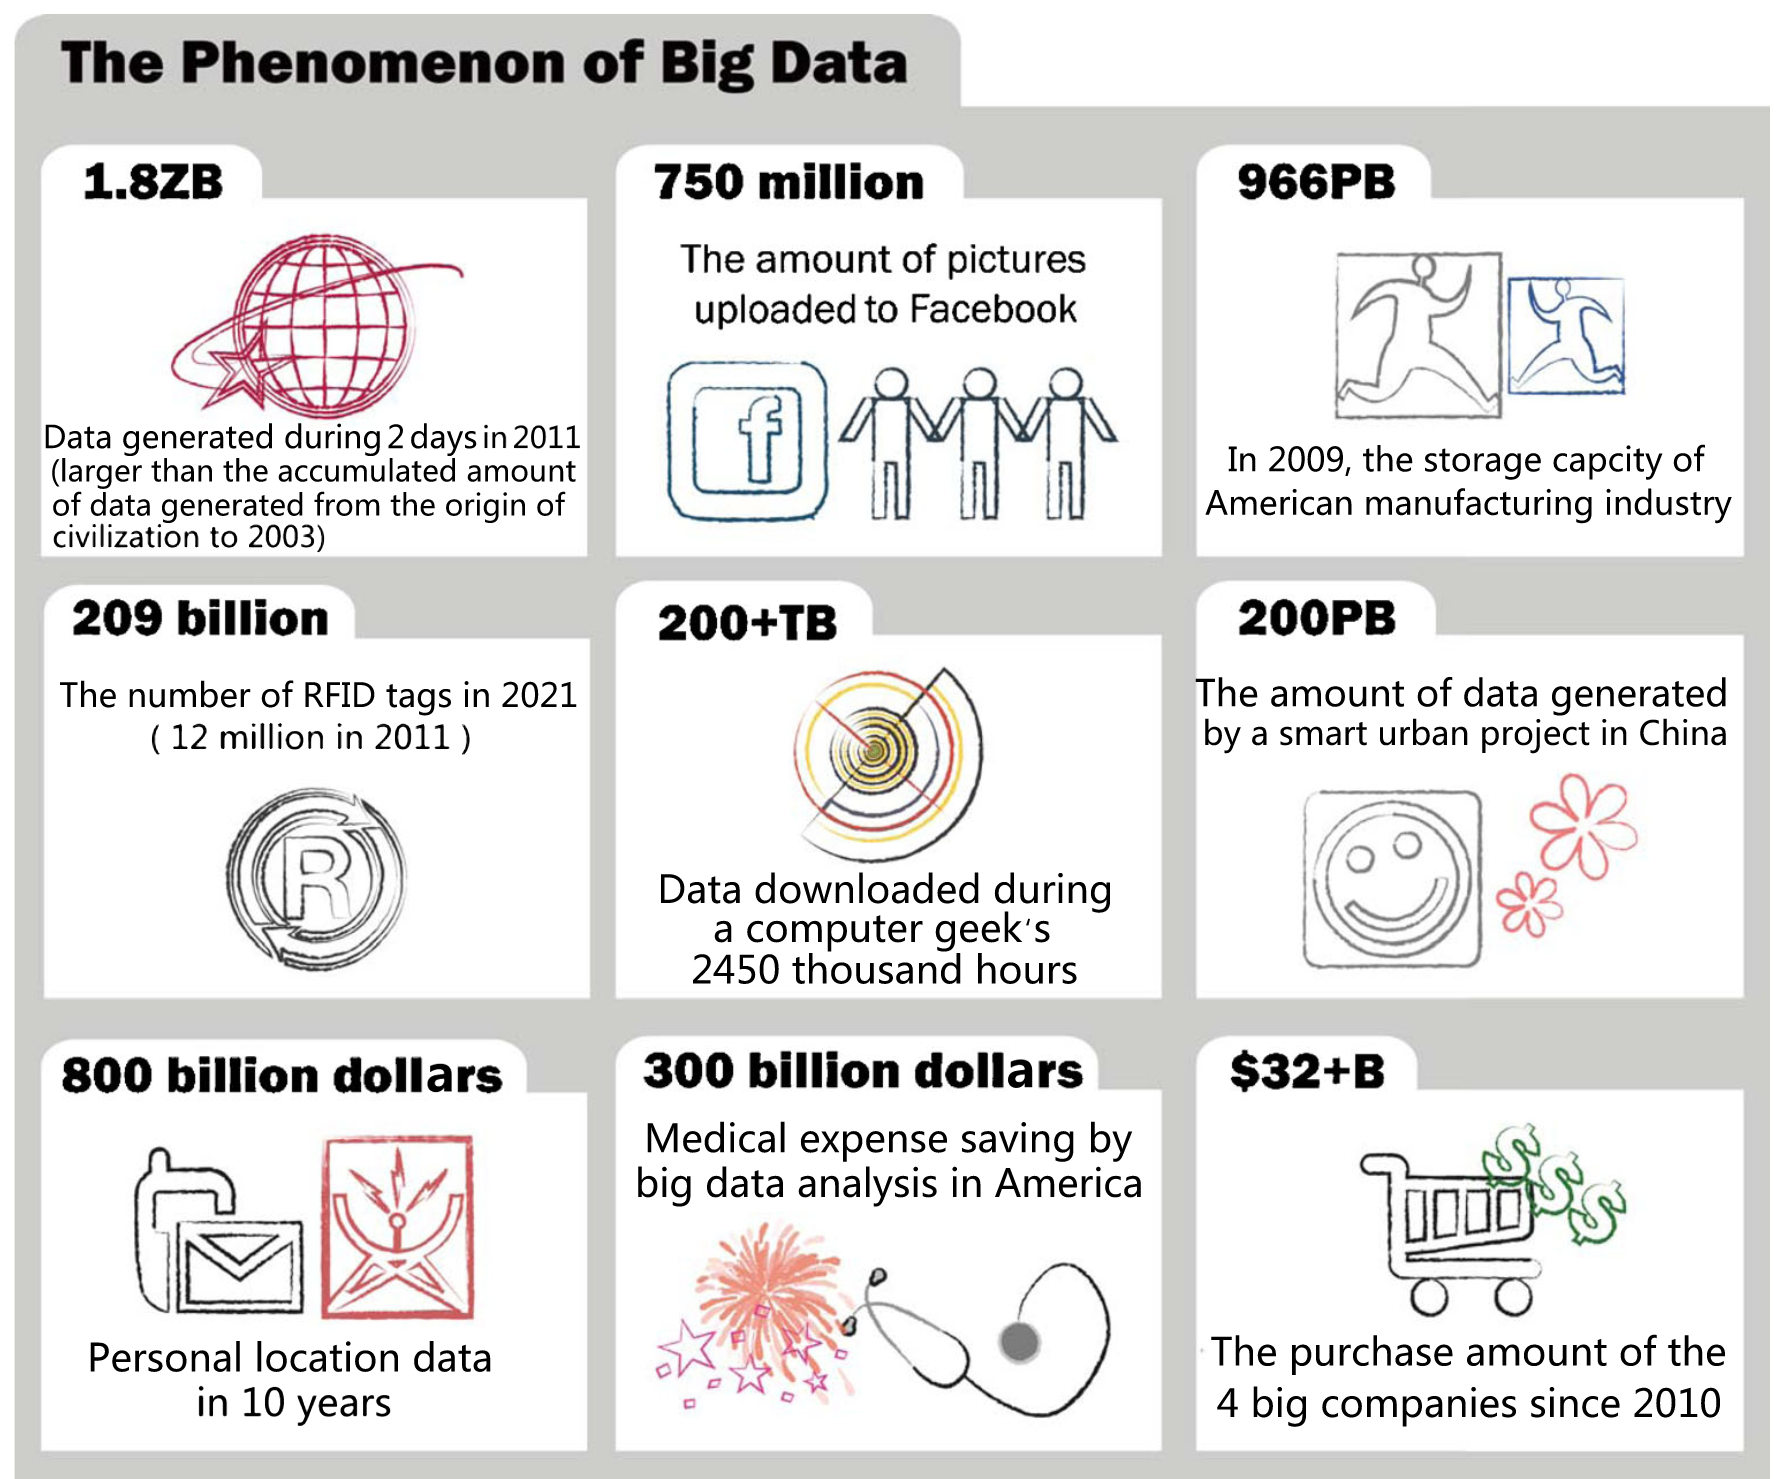
\includegraphics[width=0.8\linewidth]{img/big-data}
	\caption[The Phenomenon of Big Data.]{The Phenomenon of Big Data.\cite{chen_big_2014}}
	\label{fig:big-data}
\end{figure}

Chen shows other examples of big data in figure \ref{fig:big-data}.

\subsection{Examples of Big Data}
Industrial equipment and engines are making use of distributed sensors that generate automated alerts when maintenance is needed\cite{destiche}.

Medicare and Medicaid are using big data predictive analytics to flag fraud before claims are paid to individuals. This has saved over \$115 million dollars a year in fraudulent payout\cite{medicaid}.

Defense Advanced Research Projects Agency (DARPA) has funded various projects for visualization battlefields in real-time and visualization and creating models for traffic flow through road networks, providing valuable intel on where to locate roadside explosives\cite{pcast}.

Researchers at the Broad Institute were able to detect genetic variants in DNA related to schizophrenia \cite{pcast}. The interesting thing about this case is that the variants were not discovered until a large number of samples were analyzed. At low numbers of sample, the variant can not be seen. At intermediate numbers of samples there is a small signal. The genetic  variants become very clear as soon as a certain threshold of data is obtained.

In a review on smart cities and big data authored by Hashem et al.\cite{hashem_role_2016}, the authors review many technologies surrounding big data and how big data can play a role in smart city infrastructures of the future. They found the following areas could benefit from using Big Data in a smart city. 

Smart grids can improve energy generation efficiency by monitoring environmental data, analyzing the power habits of users, and measuring consumption from smart meters\cite{lai2015big}. Smart grids can also make use of big data to perform forecasting of future load generation\cite{al2015applications}. 

Healthcare is another sector that can gain insights on the back of big data. One healthcare project monitored and cross correlated sensors in a neo-natal intensive care unit in order to identify factors that could lead to an infection or early warning signs of infections. Data that was collected included temperatures and heatrates. Analysis allowed doctors to make diagnosis that they would have missed otherwise without big data analytics\cite{ibm_healthcare}.  Analytics of big data in healthcare using big data mining techniques can be used for diagnosing patients, predicting illnesses, and predicting epidemics\cite{roy2007middleware}.

Smart cities can make use of big data to decrease traffic congestion and better plan freight management by analyzing real time traffic sensors and using predictive analysis to determine traffic routes ahead of time\cite{ADMA}. Of course, Google and other companies already do this by analyzing mobile devices to determine and predict traffic congestion.

Hashem et al.\cite{hashem_role_2016} cite several examples of succesful smart city projects in Stockholm, Helsinki, and Copenhagen.


\section{Cloud Computing} \label{sec:cloud-computing}
NIST\cite{mell2011nist} defines cloud computing as ``a model for enabling ubiquitous, convenient, on-demand network access to a shared pool of configurable computing resources (e.g., networks, servers, storage, applications, and services) that can be rapidly provisioned and released with minimal management effort or service provider interaction''.

The major five tenants of cloud computing as defined by NIST are as follows: 

\textit{On-demand self-service} where the user can provision network, storage, and compute capacity automatically without the need for human intervention. In essence, this becomes a virtual shopping mart where to the consumer it appears that virtually unlimited cloud resources are available to chose from and the user (or algorithm) can increase or decrease the utilization of cloud resources at any time.

\textit{Broad network access} where computation capabilities are performed over a network and results are delivered to clients such as mobile devices. 

\textit{Resource pooling} where resources within a cloud such as storage, network, or compute capacity are shared among multiple tenants. This allows for efficient utilization of hardware when generally virtual services are provided to clients. Clients don't necessarily know where their physical hardware is located or provisioned. 

\textit{Rapid elasticity} is the ability to provision or remove cloud resources (i.e. storage, network, or compute resources) at any time from a system as demand on that system either increases or shrinks. Often times a human may not even be involved in making these decisions and this scaling will take place automatically using a set of predefined usage thresholds.

\textit{Measure service} where cloud providers provide a means of metering the compute resources that are used by clients. This provides a transparent means of selling cloud computing resources to clients and clients can always know how much capacity they have consumed.

Even though the NIST definition is starting to show its age, its major tenants are still the underlying foundation of cloud software even today. Many additional service and deployment models have been developed since NIST defined cloud computing, but an understanding of the basic underpinnings is required before exploring the rest of this vast filed.

Cloud computing frameworks can provide on-demand availability and scaling of virtual computing resources for storage, processing, and analyzing of very large data sets in real-time or near real-time. This model makes it possible to build applications in the cloud for dealing with Big Data sets such as those produced from large distributed sensor networks.

By using the cloud as a central sink of data for our devices within a sensor network, it's possible to take advantage of central repositories of information, localized dynamic computing resources, and parallel computations.  With the advent of cheap and ubiquitous network connections, it's becoming easier to do less processing within sensor networks and to offload the work to a distributed set of servers and processes in the cloud\cite{kamburugamuve_framework_2015}.

Cloud computing includes both technical and economical advantages as discussed in \cite{botta_integration_2016}. 

On the economical side, computing resources are pay-per-use. Businesses can dynamically increase or decrease the computing resources they are currently leasing. This makes it possible to utilize massive amounts of computing power for short amounts of time and then scale back resources when demand isn't at its peak. Before cloud computing these same businesses would be required to manage and maintain their own hardware for peak load without the ability to dynamically scale their hardware if the peak load were to increase.

On the technical side, the localization of computing resources provides for a wide variety of benefits including energy efficiency, hardware optimizations, software optimizations, and performance isolation. 

% Other advantages of cloud computing for mobile devices and data
% maybe a brief forway into fog and jungle computing
% The cloud as a collection of services
\subsection{Cloud Computing Service Models} \label{ssec:cloud-computing-service-models}
When discussing cloud computing, it's useful to understand the service models that traditional cloud computing provide. The three major service models as defined by NIST\cite{mell2011nist} are \textit{Infrastructure as a Service} (IaaS), \textit{Platform as a Service} (PaaS) and \textit{Software as a Service} (SaaS).

At the lowest level is  the Infrastructure as a Service (IaaS) model which provides virtual machines that users have the ability to  deploy and manage. Users can install operating systems on these virtual machines and interact with deployed virtual machines as if they were local servers.  Consumers using IaaS have the ability to manage and provision virtual hardware and network resources, but do not need to worry about the underlying hardware or network infrastructures. Other than providing virtual resources, consuming utilizing IaaS still require a decent amount of systems administration knowledge develop, deploy, and secure applications into the cloud using IaaS.

Sitting in the middle of the traditional cloud service models is the Platform as a Service (PaaS)  model. In this service model consumers don't have the ability to interact or provision individual cloud resources such as virtual machines, storage, networking, or compute capacity. Instead, users have the ability to deploy their application to the cloud via custom cloud provides tools or via a cloud provided application programming interfaces (APIs).

At the highest level is the Software as a Service (SaaS) layer. Generally speaking, applications in a SaaS environment are generally provided by the cloud provider. In a SaaS model, users do not have the ability to control their own cloud resources and users do not have the ability to upload their own applications to the cloud. Users do sometimes have the ability to alter the configuration of the software they are interacting with in this model.

Since the original service models were penned, there have been many other types services models introduced. Several of these focus on IoT service layers as noted by Botta et al's\cite{botta_integration_2016}. These include \textit{Sensing as a Service} (S$^2$aaS), \textit{Sensing and Actuation as a Service} (SAaaS), \textit{Sensor Event as a Service} (SEaaS), \textit{Sensor as a Service} (SenaaS), \textit{Data Base as a Service} (DBaaS), \textit{Data as a Service} (DaaS), \textit{Ethernet as a Service} (EaaS), \textit{Idendity and Policy Management as a Service} (IPMaaS), and \textit{Video Surveillance as a Service} (VSaaS).

Some of the above mentioned service models are of particular interest for a survey examining cloud computing and sensor networks. We will examine these in more detail in sections \ref{ssec:sensing-as-a-service}.

\subsection{Sensing as a Service} \label{ssec:sensing-as-a-service}
Sensing as a Service (SaaS or S$^2$aaS) describes ``the process of making the sensor data and event of interests available to the clients respectively over the cloud infrastructure''\cite{dash_survey_2010}. 

The sensing as a service model includes 4 layers\cite{perera_sensing_2014}. Figure \ref{fig:sensing-as-a-service} shows these 4 layers in more detail.

\begin{figure}
    \centering
    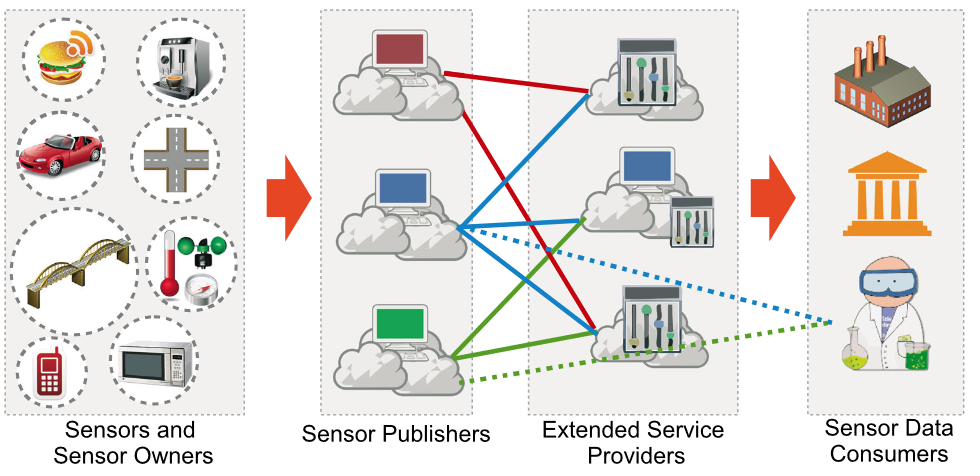
\includegraphics[width=1.0\linewidth]{img/sensing-as-a-service}
    \caption[Sensing as a service layers.]{Sensing as a service layers.\cite{perera_sensing_2014}}
    \label{fig:sensing-as-a-service}
\end{figure}

The \textit{sensor and sensor owners} layer includes physical sensors which can sense an increasingly broad variety of natural phenomena and sensor owners which can be personal, household, private, public, or commercial. Sensor owners have the final say in what data gets to the cloud and who can access the data once it is in the cloud using conditions and restrictions.

The \textit{sensor publishers} (SP) layer manages the detection of online sensors and acts as a middle-man between sensor consumers and sensors and sensor owners. Sensors register with the publisher layer. Sensor data consumers make requests to sensor publishers for specified types of data over specified amounts of time.

The \textit{extended service providers} (ESP) layer builds abstraction on top of sensor publishers. A single ESP can interact with mulitple SPs. ESPs can be used to automatically request data from multiple sensors depending on criteria provided to the ESP. This can be useful if the sensor consumer does not care about the underlying individual sensors but instead queries data at a higher level (i.e. all temperature data within a given polygon).

Finally, the \textit{sensor data consumers} layer consist of data consumers who must register with the ESPs and provide valid digital certificates. Consumers can either deal with SPs directly or deal with ESPs. The benefit to dealing with SPs is reduced cost of communications with the ESP. The benefit of dealing with ESPs is higher level querying to data and the ability to query data across multiple SPs.

I find sensing as a service appealing, but lacking in actual implementation details. To Perera's credit, he does mention quite a few open technological challenges that need filled including architectural designs, sensor configuration, sensor management, data fusion, filtering, processing, storage, and energy consumption.

Rao et al.\cite{rao_cloud_2012} mention several other research challenges for SaaS including the need for a standard distributed computing framework for distributed big sensor data as well as a framework for the real-time monitoring of sensor events.

\subsection{Sensor as a Service} \label{ssec:sensor-as-a-service}
In a Sensor as a Service (SenaaS) \cite{alam_senaas_2010} service model, virtual and physical sensors are combined according to a Service Oriented Architecture. This type of model concerns itself more with the management of distributed sensors than it does with the access, transfer, and governance of data as the sensing as a service model\cite{zaslavsky_sensing_2013}. Figure \ref{fig:sensor-as-a-service} shows the three layers that make up the architecture in the SenaaS model. Sensors and events can be defined and standardized in XML and other serialization formats such as SensorML\cite{sensorml} and OWL\cite{dean_owl_2004}.

\begin{figure}
    \centering
    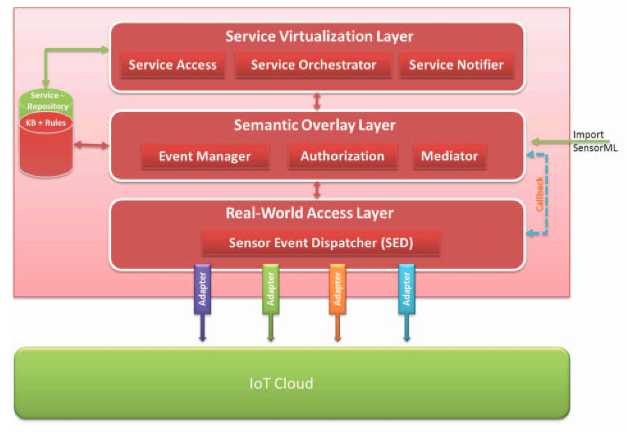
\includegraphics[width=1.0\linewidth]{img/sensor-as-a-service}
    \caption[Sensor as a service layers.]{Sensor as a service layers.\cite{alam_senaas_2010}}
    \label{fig:sensor-as-a-service}
\end{figure}

The \textit{Real-World Access Layer} interfaces to the sensors using adapters which need to be designed for each sensor. Messages from this layer are asynchronously forwarded to the \textit{Semantic Overlay Layer} via callbacks.

The \textit{Semantic Overlay Layer} is responsible for persisting data either in-memory or on disk. This layer also provides for in-memory caching capabilities. Policy based authorization can be implemented in this layer to provide some control over data access.

The \textit{Service Virtualization Layer} provides an abstraction on top of the semantic overlay layer by performing queries based on the access rights of consumers. This layer transforms the results of queries into something that can be consumed by the clients.


\subsection{Cloud Deployment Models} \label{ssec:cloud-deployment-models}
NIST\cite{mell2011nist} provides four types of deployment models in its cloud computing definition: \textit{private cloud}, \textit{community cloud}, \textit{public cloud}, and \textit{hybrid cloud}.

A private cloud is is a cloud where resources are provisioned to a single organization (or multiple parties within a single organization). In this model the organization may deploy their own cloud hardware or use cloud resources provided by a third party.

In a community cloud, resources are provided to a group of organizations that have similar requirements and may be owned and managed by a single organization, multiple organizations, or third parties.

Public clouds provide computing resources to anyone willing to purchase  said cloud resources. Public clouds can be owned and manged by anyone, a government, or any third-party. Generally all hardware in public clouds are managed by the cloud provider.

Hybrid clouds use and provide a combination of the previously mentioned deployment models and can be configured, split-up, and manged in many ways.

Virtual private clouds as described in Botta et al.\cite{botta_integration_2016} provide aspects from both public and private clouds using virtual private network (VPN) technology to allow users to manage specific and often times complicated network technologies.

\subsection{Mobile Cloud Computing} \label{ssec:mobile-cloud-computing}
Mobile cloud computing (MCC) combines mobile computing, cloud computing, and data analytics\cite{wang_mobile_survey_2015}. Mobile devices such as smartphones make fantastic distributed sensors for temporalspatial data. Not only do they carry a wide array of sensors on-board (microphones, barometers, accelerometers, GPS, compasses, cameras, clocks), but they generally have multiple modes of offloading data (WiFi, bluetooth, cellular, SD cards), and support some pre-processing on the device. Advances and expansion of wireless technologies make it increasingly feasible to connect wireless devices to the network and offload computation and analytics to a scalable and distributed backend\cite{barbera_offload_2013}.

Mobile devices, which are power, compute, and memory constrained can take advantage of uploading data to the cloud for persistence and analysis. Once data is in the cloud, analytics can take advantage of the fact that the cloud can integrate data from many sensors (and other data sources), creating a real-time global view of the network.

Existing MCC application domains include mobile commerce, mobile sensing, mobile banking, crowdsourcing, mobile healthcare, and augmented/virtual reality.

Crowdsourced data capture was an early application of MC\cite{campbell_rise_2008} and continues to be a main driver of MCC. One example of this is an application, that during amber alerts, allows users to upload pictures to the cloud where thousands of photographs can be analyzed in parallel, helping to track down missing children\cite{satyanarayanan_mobile_2010}.

Collective sensing and location based services are other major drivers of MCC. Collective sensing takes advantage of the sensors on mobile devices to get a global view of some physical phenomenon. Common sensors that are used in mobile sensing includes microphones, barometers, WiFi chipsets, GPS, and others. Examples of mobile sensing include distributed weather gathering, acoustic classification like Lu et al.'s\cite{lu_soundsense:_2009} SouneSense framework which uses distributed Apple iPhones to classify audio events. There has been a surge of research relating to predicting and analyzing real time traffic congestion \cite{thiagarajan_vtrack:_2009}, \cite{herring_using_2010}, \cite{hunter_scaling_2011}. 



\subsection{Issues with Cloud Computing} \label{ssec:issues-with-cloud-computing}
The biggest issues facing cloud computing deal with security and privacy. Subashini et al.\cite{subashini_survey_2011} go into the specific security and privacy risks associated with the three major cloud deployment models. The following is largely a review of their work. 

The deployment model that exhibits the most risks in the PaaS layer since this model requires that consumers manage their own virtual machines, deployment of cloud applications, and configuration. Within this model, the following items are of concern. 

Data security is a concern on all deployment models, but especially at the PaaS layer where sensitive data will be stored on remote servers not owned by a client. Since clients manage their own servers in the PaaS layer, they are also required to manage their own data security. Data security issues include cross-site scripting, access control weaknesses, injection attacks, cross-site request forgery, cookie manipulation, hidden field manipulation, insecure storage, and insecure configuration.

Network security becomes an issue when sensitive data is transferred from clients to the cloud backed and visa-versa. If encryption is not used, users could be vulnerable to port scans, ip spoofing, man-in-the-middle attacks, packet sniffing, and more. Even if encryption is used, users can still be vulnerable to packet analysis, insecure SSL configurations, session management weaknesses.

Laws and regulations often require that data not leave or enter certain jurisdictions giving rise to issues of data locality. Users generally do not get to decide where data is stored within a cloud environment as most of those decisions are handled by the cloud provider.

The introduction of distributed systems means that we can no longer make guarantees about data persistence such as ACID (Atomicity, Consistency, Isolation, Durability). Without these guarantees a large amount of data integrity issues surface. We will look at these issues in greater detail when discussion big data persistence models in later chapters.

Data segregation issues occur with multiple virtual resources sharing the same physical resources. Data can be unintentionally leaked or stolen either by attacking the cloud provider multi-tenancy framework or by attacking the virtual servers directly through SQL injection, data validation, and insecure storage.

Large organizations with multiple employees having access to the cloud can create data access issues. Clear policies must be defined, enforced, and updated as to which virtual resources employees have access to. 



At some level, consumers are required to trust that the cloud provider they choose will implement security and privacy best practices within their cloud architecture. This does now however resolve the larger issues of security vulnerabilities within cloud software and their communication components.

% Something about runaway data costs.... there was an issue once of someones AWS key being found and then their servers got pwned and were used for generating bitcoin or something


%%%%%%%%%%%%%%%%%%%%%%%%%%%%%%%%%%%%%%%%%%%%%%%%%%%%%%%%%%
\section{Big Data Persistence Models} \label{sec:big-data-persistence-models}
Traditional storage methods for meta-data and related products has traditionally made use of the filesystem and relational database systems (RDMS).

Big data by its nature can be structured, unstructured, large, diverse, noisy, etc. Many of the properties of big data do not fit nicely into the structured world of traditional RDMSs.

In-order to meet the needs of big data and distributed sensor networks, we look to the ever growing field of NoSQL (not only SQL) and related Big Data storage models. There are multiple types of data models with different use cases.

According to Song et al.\cite{5980904} an ideal NoSQL data model strives for ``high concurrency, low latency, efficient storage, high scalability, high availability, reduced management and operation costs.'' The challenges of realizing an ideal NoSQL data model however lie in three main areas\cite{chen_big_2014}: consistency, availability, and partition tolerance. 

% Discussions on consistency
Several of the persistence models we review do not support ACID (Atomicty, Consistency, Isolation, Durability). A consequence of this is less than perfect consistency. Consistency issues occur when data is stored in a distributed manner with multiple copies. In situations of server failure (or with systems that support different consistency models), situations can arise where multiple copies of the same resource contain different contents. 

Vogels and Wener\cite{vogels_eventually_2008} explain the main forms of consistency. Assume a record is being updated across multiple servers. With ``strong consistency'', any access of that resource after the update will return the updated result. With ``weak consistency'', subsequent access of that resource is not guaranteed to return the updated result if that access is within a certain ``inconsistency window''. With eventual consistency, the only guarantee you get is that access to the resource will be show up ``eventually'' where eventually can depend on many factors.

% Discussions on availability
As the amount of hardware (servers, switches, \textit{etc}) increases in a distributed system so does the amount of hardware errors. Availability refers to the ability to remain operational even as parts of a distributed system drop in and drop out\cite{chen_big_2014}. Gilbert\cite{gilbert2002brewer} defines availability as ``every request received by a non-failing node in the system must result in a response." He goes on further to point out that this definition does allow for unbounded computation since it's possible to wait for a result that never returns.

% Discussion on partition tolerance
As the amount of hardware increases in a distributed system, the number of communication packets that drops also increases. The ability to maintain service in the face of some amount of drops refers to partition tolerance\cite{chen_big_2014}.

The above ideas are all tied together into the CAP theorem proposed by Brewer\cite{brewer2000towards} which states that in any shared data system, you can only achieve two of the three following properties: Consistency, Availability, or Partition (tolerance). As we review different Big Data architectures, we will examine how they fit into the CAP theorem and what guarantees they provide for these three major areas of distributed data management.

We also believe, ease of use, maturity of the product, and community (or commercial) support should also factor into the comparisons between data models. 

With the above factors in mind, we can begin categorizing and analyzing several major Big Data model solutions.


\subsection{Distributed File Systems}
Before we look at specific big data storage systems, we will first examine how to store big data using file systems as file systems provide the base storage backend for distributed storage applications. Distributed file systems are not a new idea. Howard et al.\cite{howard_scale_1988} describe the scale and performance issues associated with Carnegie Mellon's distributed Unix based \textit{Andrew File System} in 1988. 

Generally, distributed file systems were developed as a means of data sharing. Big data however, with the characteristic of large volume, often doesn't fit on a single disk, or a single machine, or a  single data center for that matter, required new techniques for storage of very massive data sets. The Google File System (GFS) was one of the first attempts at storing big data using a distributed file system. For that reason, this review will focus on technologies from GFS and onwards. 

\subsubsection{Google File System (GFS)}
Ghemawat et al. at Google introduce \textit{The Google File System}\cite{ghemawat_google_2003} in 2003. Google wanted to design a distributed file system that not only provided scalability, availability, reliability, and performance, which is something that previous distributed file systems could do, but to design it in such a way that it meets the needs of a big data world. 

The authors note that in large distributed systems comprised of commodity hardware, failure is the norm rather than the exception. GFS is designed in a way to provide monitoring, error detection, fault tolerance, and automatic recovery of distributed data. 

Google noticed that files were becoming much larger and multi-gigabyte sized files were becoming common and should be prioritized. The volume of small files also continued to increase into datasets terabytes in size consisting of billions of small files. GFS examines traditional I/O patterns and block sizes.

The authors stated that there were common read/write patterns among services in their cluster. Reads generally consisted of large streaming reads of small random reads. Writes generally consist of large sequential writes. Once written, files are often not written to again. Small writs are supported, but not prioritized. 

GFS prioritizes the ability for multiple clients to append to the same file concurrently in an efficient with minimal synchronization overhead.

Finally, GFS should prioritize high bandwidth over low latency with the assumption that most use cases require processing bulk data at a high rate.

GFS provides a non-POSIX but familiar interface utilizing a directory/file hierarchy and supports creating, deleting, opening, closing, reading, and writing of files.

A GFS system consists of a single master node and multiple chunk servers. Files stored on GFS are divided into fixed-size 64 megabytes chunks and replicated a configurable amount of times on multiple chunk servers. The single master node coordinates locations of chunks in the systems, but only provides routing information. The master node hands off clients to chunk servers to read and write to directly. A chunk block size of 64 MB provides the benefits of less routing requests to the master node and reduces the amount of meta data stored on the master.

The master node keeps track of three types of metadata: file and chunk name spaces, mapping from files to chunks, and locations of chunk replicas. All metadata is stored in memory so that access and manipulation is efficient. The master's metadata transformations are written to an operations log and stored locally as well as remotely and allows for replacing the master in the event of a failure.

The master has several other responsibilities as well. The master is in charge of optimizing replica placement by considering reliability, availability, bandwidth utilization. The master also takes into account the health of the servers that chunks are on including disk utilization. The master can re-replicate chunks when other chunks fail and also rebalance chunks in order to optimize reliability, availability, bandwidth utilization. Files are not immediately deleted. They are marked deleted, but their contents are cleaned up at a later time during a garbage collection phase coordinated by the master.

Similar to other distributed systems, GFS can not make full ACID guarantees and uses a relaxed consistency model. The master node handles namespace mutations (i.e. file creation) and locking so that these operations are atomic. Mutations to files from multiple clients can cause consistency issues when overwriting or inserting into a file. Appends to a file can be made to be atomic if the client does not specify an offset and instead allows GFS to perform the append. Replicas are updated in the same order on all machines so that in general they should all have the same state at the same time. There are instances during failure or when clients cache chunk locations and read from a stale replica where they may retrieve old or inconsistent data. 

GFS provides almost instantaneous snapshot capabilities which can be used to create copies, divergent branches of data, or create data checkpoints. Snapshots are created using copy-on-write techniques where if data is not changed, copies can simply point to the original data source, but anytime the original copy changes, a new copy is created. Hence, copies are deferred to first write. 

In an interview with Sean Quinlan\cite{mckusick_gfs:_2010} (2010), one of the lead architects of GFS, Quinlan discusses how GFS has changed in the 7 years since its conception. 

The biggest change they made to GFS was the creation of a distributed master system rather than a single master. This change came about when data volumes grew initially from tens of terabytes to tens of petabytes in the span of a couple of years. The overhead of meta-data became too great for a single massive master server to handle. Even though clients rarely interact with the master server, something as simple as creating a file could end up in a queue with thousands of other client requests as well. Google decided to build a distributed master server network initially by placing a master server per data center and later multiple master servers per data center. Each master can index 100 million files in memory and there are hundreds of masters.

A major issue that Google ran into internally with GFS was bottle necks due to the volume of small files some projects used. Each file in GFS has meta-data associated with its namespace and the locations of its chunks. The overhead of meta-data caused by many small files was so substantial that Google mandated that applications must find a way to store there information in larger chunks of data and put a quota on the number of files an individual client can create.

As applications changed at Google from batch processing jobs that could take hours to run to a need for more real-time data for user applications, it was clear that Google's previous focus on optimizing for throughput rather than latency needed to change. One solution to this at the GFS level is to leverage parallel writes and perform merges later. In this scenario, if a single write hangs or fails, one of the N parallel writes may succeed. By leveraging parallelism, applications utilizing GFS can give the impression of low latency. Distributed masters also help with latency when performing operations on the file system.

Quinlan concedes that the initial design of relaxed consistency did cause many issues with some of there users down the road and that if he could redesign GFS he push to serialize writes from multiple clients that can ensure replicas remain consistent.


\subsubsection{Hadoop Distributed File System (HDFS)}
The Hadoop Distributed File System (HDFS), described by Shvachko et al in their 2010 paper, \textit{The Hadoop Distributed File System}\cite{shvachko_hadoop_2010}, is a file system designed for storing big data across a distributed set of servers. HDFS was heavily influenced by GFS and aims to provide an open source alternative to GFS. HDFS acts as the backbone for a myriad of big data persistence and big data analytics frameworks including Spark, MapReduce, HBase, Pig, Hive, ZooKeeper, Avro, Chukwa, and others. A full list of software that integrates with HDFS is maintained at \url{https://hadoopecosystemtable.github.io/}\cite{hadoop-ecosystem}. 

As mentioned previously, HDFS is heavily influenced by GFS. Therefor, this review of HDFS will look at the main comparisons between the two distributed file systems, drawing comparisons from Vijayakumari's 2014 comparison paper\cite{vijayakumari_comparative_2014}. The design goals of HDFS and GFS are largely the same. Support for management of large files as part of large data sets, support for batch computing and big data analytics, and high data availability.

HDFS refers to its meta-data servers as \textit{name nodes} and it data servers as \textit{data nodes} compared to GFS's \textit{master nodes} and \textit{block nodes}.

GFS and HDFS both store data using a hierarchy of files and directories. However, the API to these file systems are not POSIX compliant and require third part APIs for accessing the file systems. HDFS further supports integration with other distributed file systems such as CloudStore or Amazon's Simple Storage Service while GFS is proprietary to Google.

Both GFS and HDFS scale using distributed clusters. Replication of data for providing availability is largely the same.

HDFS uses a permission model that is similar to the POSIX model where files and directories can have separate permissions for owners, groups, and other members. GFS uses a proprietary permission model within its organization that is not based off of POSIX permissions.

GFS and HDFS alike store data in chunk sizes of 64 MB where this value can be configurable. GFS makes use of the Linux kernel's buffer cache to keep frequently accesses data in memory while HDFS uses a combination of a public and private distributed cache. A key difference between the two is that the GFS master node provides clients with the location of blocks where HDFS exposes block locations to allow application to schedule tasks bases on where content is within the distributed system.

GFS uses TCP to communicate between servers and HDFS uses an RPC protocol on top of TCP.

Both of these file systems server similar roles, but HDFS has a much larger impact on the academic realm due the the sheer number of other applications and frameworks that build on top of it.

\subsubsection{Haystack}
Beaver et al. at Facebook describe a distributed object storage system for storing petabytes of photographs in their 2010 paper \textit{Finding a Needle in Haystack: Facebook's photo storage}\cite{beaver_finding_2010}. As of 2010, Facebook had stored over 260 billion images.

Haystack was designed to provide high throughput rather low latency and allow Content Delivery Networks (CDNs) to deal with caching and latency issues. Similar to the other distributed file systems, Haystack also wants to provide fault tolerance with the statistical likelihood of software and hardware failures. Another requirement for Haystack is that it is cost-effective along the dimensions of cost per terabyte and normalized read rate. Haystack claims cost per terabyte are 28\% less than a similar NFS solution and provides 4x more reads per seconds than a similar NFS based approach.

CDNs are able to cache the most recently accessed photos, but Facebook noticed a pattern where older photos are also accessed frequently. This resulted in a large amount of cache misses on Facebook's CDNs. Cache misses originally resulted in making requests to NFS shares where each directly contained thousands of photos. The number of seeks required to find a single photo started to become a bottleneck. Taking inspiration from GFS, Facebook created Haystack as a distributed object store focuses on storing and managing its billions of photographs.

Haystack is split into three components. The \textit{Haystack Store}, \textit{Haystack Cache}, and \textit{Haystack Directory}.

The Haystack Store is the main improvement Haystack brings to the table compared to the NFS approach is that Haystack stores individual photos and metadata, called ``Needles" into a large (on the order of 100 GB each) continuous files (see figure \ref{fig:haystack}). By using large files instead of many individual files, they can reduce the amount of disk accesses required to find and load individual photographs. 10 TB servers are split into 100 physical volumes of 100 gigabytes each. Each physical volume resides on a single machine, but logical volumes can span multiple machines and multiple physical volumes. When a photo is written to the store, it is stored in a single logical volume, but duplicated multiple times over physical volumes to provide availability. The backing filesystem is XFS which provides small enough blockmaps that they can be stored in physical memory as well as efficient file preallocation. The store also keeps an index file that allows the in-memory mappings to be recreated on failures or server restarts without having to read through the entire file system.

A service called Pitchfork is used to continuously monitor, detect, and repair services in Haystack. In the event of failures, new servers can be brought online and data can be synchronized from the replicas.

\begin{figure}
	\centering
	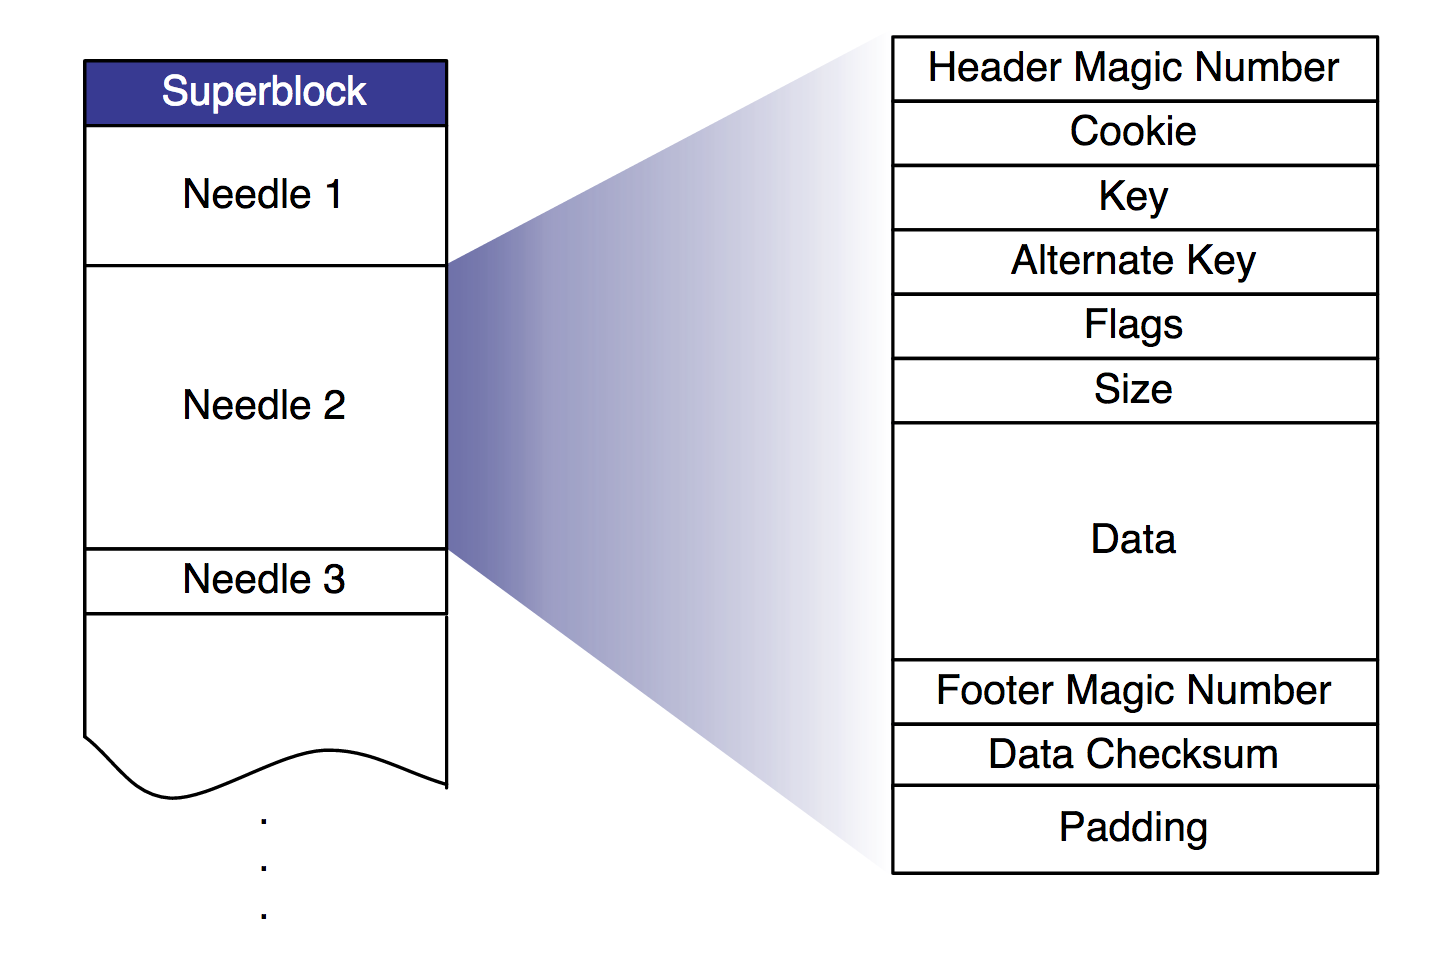
\includegraphics[width=1.0\linewidth]{img/haystack}
	\caption[Haystack individual file layout.]{Layout of Haystack Needle within a physical volume.\cite{beaver_finding_2010}}
	\label{fig:haystack}
\end{figure}

The Cache component provides an intermediate layer of photo caching between CDNs and the Haystack Store. Requests for photos contain three URLs. The first URL is a lookup key for the data in the CDN. If the CDN does not have the image cached, the CDN URL is stripped and the photo request is forwarded to the Haystack cache. Again, if the photo is not found in the cache, the Haystack URL is stripped and the request is forwarded to the Haystack Store. These requests are made over HTTP and the format of the requests are as follows: $http://<CDN>/<Cache>/<Machine Id>/<Locaical Volume, Photo>$.

The Haystack Directory servers provide mappings from logical volumes to physical volumes. They are also in charge of determining whether a read photo should be stored in the Haystack Cache or in a CDN cache. Finally, Haystack Directory servers provide load balancing for writing across logical volumes and reading across physical volumes.

On-top of these three services, Haystack provides a small set of other improvements including compaction which reclaims space of deleted photos and custom binary encoding of indexes to improve space efficiency. In the end, Facebook was able to improve on their photo storage and management by showing performance and efficiency gains over their previous NFS based approach.

TODO: Find a way to summarize

\subsection{Key-Value}
The simplest data model for distributed storage is likely the Key-Value (KV) data model \cite{weber_nosql_2010}. In this model, every piece of data stored is indexed by a unique primary key. Queries to that item all happen via its key to access the value. Values in a KV system can be treated as blobs and the content of the value is irrelevant to the semantics of KV stores. KV systems are popular due to their simplicity and ease of scaling.

Keys in KV systems are the unit parallelism that provide the main means of concurrency. If you want to guarantee transactions, then keys can be naively sharded across servers. This does now however provide safety of data loss in which case a system will strive to provide replication at the cost if ACID compliance. Stores and requests can usually be achieved in $O(1)$ even in distributed systems\cite{ravendb}.

If the major advantages are simplicity and query response time\cite{chen_big_2014}, the major disadvantage to KV stores is the fact that they lack advanced query capabilities. The only way to query a database is by its unique key. Range based queries, secondary, and tertiary indexes are only supported by a third party systems or application code. Joins can only be performed in application code\cite{design-voldemort}.

Popular KV based solutions include Dynamo, Riak, Voldemort, Redis, MemcacheDB, Ignite and others.

\subsubsection{Memcached}
One of the earliest examples of a distributed KV store is memcached\cite{fitzpatrick_distributed_2004} which was created in part to power the dynamic content of 70 distributed LiveJournal servers. The developer, Fitzpatrick, believed that scaling out on many tiny machines rather than up was the appropriate response for increased data loads. Even though they had SQL database clusters, they could not provide caching on those machines in front of the database due to limitations in address space (32-bit). Fitzpatrick realized that there is a lot of spare memory on the network, even if in small chunks, so the dream of a distributed KV store as a cache was born. Memcached had no persistence guarantees. If a server went down (hardware or software), the data would simply be deleted and any requests to that data would result in a cache miss. Since memcached is used for caching, this is not a huge concern. The real benefit of distribution is that if one server goes down, not all data is lost. It also allows users to take advantage of memory from multiple servers, which wasn't easily possible before.

\begin{figure}
    \centering
    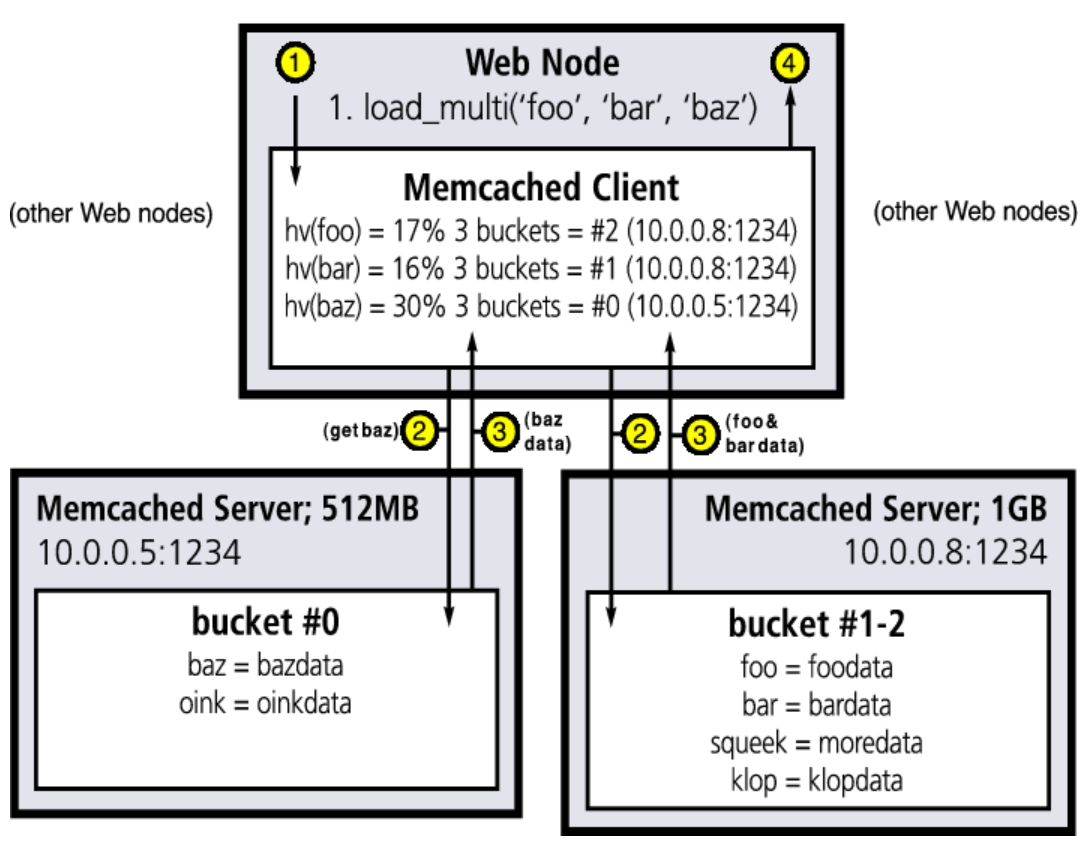
\includegraphics[width=1.0\linewidth]{img/memcached}
    \caption[Mecached architecture.]{Mecached architecture. \cite{fitzpatrick_distributed_2004}}
    \label{fig:memcached}
\end{figure}

Memcached is architected as a 2-way hash-table as show in figure \ref{fig:memcached}. The first layer of hashing takes place in the client library. When a client receives a lookup request for a key, that key could live on any of the memcached server instances. The client hashes the key to determine which server the data is actually on. The request if forwarded to the appropriate server, and the server performs a hash lookup on the provided key and either returns a result or creates a cache miss. This system generalizes to a distributed hash table and provided $O(1)$ lookups and stores. Memory is allocated using slab allocator which used a free list to keep track of free chunks inside of slabs. The protocol allows for fetching multiples keys at one time. 

TODO: Review Scaling Memcache at Facebook

\subsubsection{Amazon's Dynamo}
In 2007, DeCandia and others working at Amazon, released their paper \textit{Dynamo: Amazon's Highly Available Key-Valye Store}\cite{decandia_dynamo:_2007}. Decandia et al. describe Dynamo as ``a highly available key-value storage system that some of Amazon's core services use to provide an 'always-on' experience''. Dynamo prioritizes availability over consistency. In order to achieve those goals, Dynamo makes extensive use of object versioning and application-assisted conflict resolution which we will look at in greater detail in the next couple of paragraphs.

As a KV store, Dynamo only provides get and put operations against a unique key and is intended to be used with small values (< 1 MB). Amazon, citing experience, mentions that ``data stores that provide ACID guarantees tend to have poor availability''. Since Amazon's goal for this data store was primarily availability, Amazon decided to use a weaker consistency model which implies that updates will eventually propagate to all peers, at some time in the future. Other guiding requirements for the design of Dynamo include: symmetry where each Dynamo process has the same set of responsibilities as all others, incremental scalability where scaling out has minimal impact on the system or its users, decentralization to avoid single points of failure, and heterogeneity where each process is tuned to the individual hardware of the server it runs on. With these design goals in mind, we next discuss how Dynamo implements these technologies.

Large distributed systems are prone to network, software, and hardware failure. To ensure high availability, Dynamo utilizes optimistic replication, where updates are propagated to $N$ peer nodes in an eventually consistent manner. All nodes in Dynamo's distributed network form a logical ring. Key's are hashed to determine a coordinator node within the ring to initially store the key value pair. The coordinator node stores the key value locally as well as on $N-1$ successor nodes going in a clockwise direction. The list of nodes that end up storing a key are called a preference list. Every node in the ring is capable of determining the preference list for any given key. Dynamo allows for gets and puts on any node in a preference list, skipping over nodes that are unhealthy. Because of this, situations can arise where there are conflicting copies of data when an update hasn't persisted to all nodes in its preference list yet. Dynamo versions all data with a timestamps to allow multiple versions of data to exist in the data store. Using semantic reconciliation, the network is usually able to determine the authoritative version. In certain failure situations where data can not be semantically reconciled, it is left up to the application to determine which value is correct.  

One of Dynamo's stated goals is to provide incremental scalability. When a new server comes online (or others go down), data must be partitioned across the new nodes. Dynamic partitioning is achieved using consistent hashing techniques as described in \cite{karger_consistent_1997}.

Gets and puts are performed in parallel on all $N$ healthy nodes in the preference list. When nodes become unhealthy, a sloppy quorum takes place and the unhealthy nodes are temporarily removed from the ring, and subsequent puts and gets happen on the successive neighbors. To protect against entire data centers going down, replicas span multiple data centers. Dynamo uses Merkle trees to detect inconsistencies between replicas and recover from permanent failures. A gossip-based protocol is used to maintain node membership within the ring.

Dynamo is used to power many of Amazon's backend services and has also been promoted as an offering of Amazon's cloud services.

Riak\cite{Klophaus:2010:RCB:1900160.1900176} is an open source implementation of Amazon's Dynamo and was built using DeCandia's paper.

\subsubsection{LinkedIn's Voldemort}
In 2012, Sumbaly and others from LinkedIn released their paper \textit{Serving Large-scale Batch Computed Data with Project Voldemort}\cite{Sumbaly:2012:SLB:2208461.2208479}. Voldemort has a similar design to Dynamo in that it utilizes consistent hashing to achieve data partitioning and replication. Clusters form logical rings, and depending on the provided replication factor, consistent hashing is used to select a subset of a cluster to replicate data on.

Unlike Dynamo, Voldemort provides (de)serialization out of the box to/from multiple formats including JSON, strings, Java byte-code, Protobuf, Thrif, Avro, and raw byte streams. Voldemort also supports tuple based compression.

One of LinkedIn's biggest features provides users with a list of people that may know by analyzing social relations between current LinkedIn friends and looking at friends-of-friends. This data is computed with a multitude of graph algorithms such as link prediction or nearest-neighbor calculations. These algorithms run over hundreds of terrebytes of offline data consisting of log files representing social networks, connections, and interactions. This graph structure changes quickly and dynamically meaning these algorithms need to run often to generate and update indexes with valid entries. 

Not only does LinkedIn need to handle very large data sets consisting of billions of tuples, they also require the ability to rollback to clean data in the presence of errors. These errors can occur during system upgrade, algorithm changes, incomplete data, or issues with a data source.

Perhaps the biggest improvement Voldemort provides over Dynamo is the ability to compute indexes offline using large distributed computation systems, mainly MapReduce, and supply partitioned data as a result of these computations. This ability allows them to refresh terrabytes of data with ``minimum effect on existing serving latency''. Voldemort also takes advantage of utilizing the operating system's page cache for efficient cache management. The collection of these improvements are referred to as \textit{read-only extensions}.

Much of LinkedIn's data can be efficiently computed offline, such as the people you may know feature mentioned earlier. Hadoop provides a map reduce model to distribute graph computations over a cluster. HDFS provides redundancy and availability of data in the face of software or hardware failure. A driver program is in charge of scheduling offline data fetches from Voldemort, map reduce runs, and swapping of live index data back into Voldemort. This process is visualized in figure \ref{fig:voldemort}. 

\begin{figure}
    \centering
    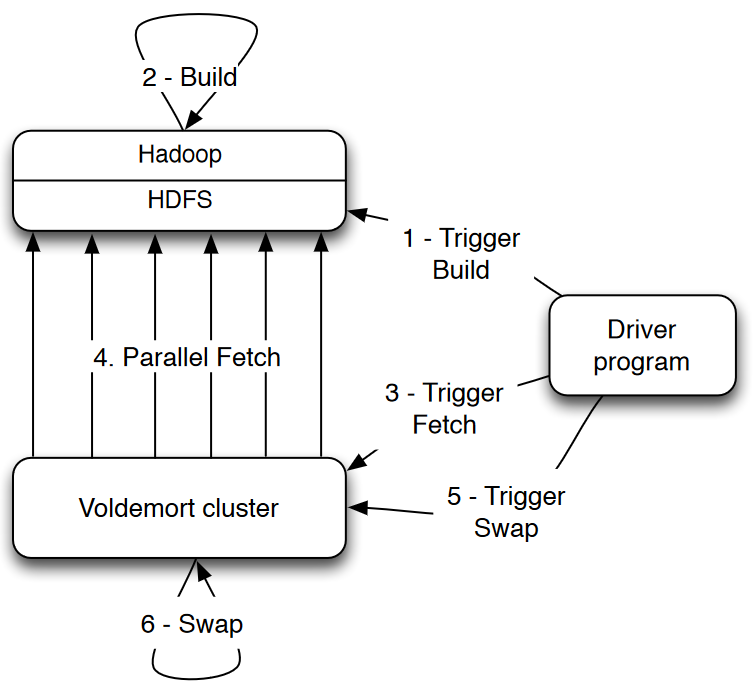
\includegraphics[width=0.7\linewidth]{img/voldemort}
    \caption[Voldemort data deployment pipeline.]{Steps involved in the complete data deployment pipeline. The components involved include Hadoop, HDFS, Voldemort, and a driver program coordinating the full process. The ``build'' steps work on the the output of the algorithm's job pipeline. \cite{Sumbaly:2012:SLB:2208461.2208479}}
    \label{fig:voldemort}
\end{figure}

Voldemort usages a storage format that memory maps indexes directly into the operating system's address space instead of creating a custom heap based data structure. Voldemort does this to allow the OS to handle caching and page caches which tend to be more efficient than custom data structures. When data is fetched from Voldemort, it is chunked and stored across HDFS in such a way that the file sizes do not become to small which Hadoop does not handle efficiently. Index files contain the upper 8 bytes of the MD5 of the key and then a 4 byte offset to the associated value in the data file. MD5 is used to provide a uniform hash space. Voldemort only uses the top 8 bytes of the MD5 to reduce the overall index size while still providing for a low amount of collisions ($\sim$.0004\%). The main advantage of this approach is that it is much more cache friendly. The downside to this approach is that there is increased complexity for dealing with collisions when they do happen.

Voldemort generates its data chunks with a single Hadoop job. The Hadoop job uses number of chunks, cluster topology, store definition, and input location on HDFS. The mapper phase of the Hadoop job partitions data based on the provided routing strategy. A three tuple of generated chunk set id, partition id, and replication factor determine how data is routed to the correct reducer. The reducer phase of the Hadoop job writes data to a single partitioned chunk set. By tuning the number of chunk sets, build phase parallelism can be configured and exploited.

Voldemort makes extensive use of data versioning. Symbolic links point to the most recent version of data on a directory. This feature makes it possible to quickly role back versions of data in failure conditions and also makes it possible to quickly updates indexes from offline data set computations.

LinkedIn continues to use Voldemort to power their people you may know data set as well as their collaborative filtering datasets. They found a 10x improvement in throughput against traditional MySQL solutions at scale. Voldemort also has smaller read latencies than MySQL. The biggest improvement comes from building data sets using MapReduce which scales linearly where the MySQL approach does not scale at all.



\subsection{Column}
Wide-column stores at first glance appear to be a regular SQL-like table turned on its side where each table contains a ``small'' amount of rows, but each row can contain a huge number of dynamic columns. Column stores are schemaless and support dynamically named columns. Generally, rows are the unit of parallelism in a column store and also the main means of distribution. 

This section will review Google's Bigtable first as most column oriented databases are inspired by Bigtable.

\subsubsection{Google's Bigtable}
2008 saw the release of Chang et al's paper \textit{Bigtable: A Distributed Storage System for Structured Data}, which describes a system developed at Google for storing structured data that has the ability to scale to petabytes across thousands of low cost commodity servers and data centers. Bigtable's stated goals are wide applicability, scalability, high performance, and high availability. Bigtable is more complex than simple KV stores and in many ways it can resemble traditional relational database management systems. Similar to the other data stores we've discussed so far, Bigtable's distrubted nature means that it can not guarantee ACID-like transactions and Bigtable relaxes its views on consistency. Bigtable is also unique in that it allows its clients to determine data locality through schema creation and whether data is persisted to memory or backed by disk. These properties allow Bigtable to provide wide applicability to a a very wide range of applications both internal to google and external through Google's cloud computing infrastructure.

Bigtable's structure can be described as ``a sparse, distributed, persistent multi-dimensional sorted map'' comprised of rows, columns, and column families. Data is indexed ny a combination of row key, column key, and 64-bit timestamp. Values in Bigtable are simple binary blobs encoded as strings forcing client side applications to make their own serialization and deserialization decisions. 

Rows are indexed by strings and reads/writes to individual rows are atomic. Ranges of rows in a table are called \textit{tablets}. Tablets are the main unit of parallelism and load balancing within Bigtable. In this structure, reads to rows can be made more efficient by keeping row ranges small and returning a small number of tablets (which generally come from a small amount of co-located machines). Each row can contain a small number of column families (on the order of hundreds), and each column family can contain arbitrarily unlimited columns. This type of data model flips the traditional row-column model of RDMSs on its head, using columns as the main means of expansion rather than rows.

Column keys are grouped into column families. Data stored in the same column family are generally related. For instance, temperature measurements could be a column family and each column inside the family is an individual measurement. Access control and memory management are performed at the column family level.

Individual stored values can have multiple versions which are sorted in timestamp order which makes tracking of updates possible. Bigtable also provides built-in mechanisms for only storing the last $N$ versions of data or to only keep data received in the last $N$ amount of time.

Bigtable's API allows for storing, querying, and deleting of data. The API allows for meta-data manipulation for access control. It's also possible to run client side scripts on the server to manipulate and filter the data similar to Redis.

Bigtable utilizes Google's distributed file system \textit{Google File System}(GFS) for log and data storage. Data is initially stored in memory, but as it grows, it will be frozen, compacted, optionally compressed, and then written to disk. Once it is on disk, it is immutable and can take advantage of gains in parallelism due to this. Bigtable provides high-availability using a distributed lock service called Chubby\cite{burrows2006chubby}. Chubby manages 5 active replicas of which one is elected to serve requests. Chubby manages consistency between replicas using the Paxos algorithm\cite{chandra2007paxos}, which is an algorithm for forming group consensus in the presence of failure. A master server is used to determine routing to and from tablet servers. However, data does not run through the master server, but directly to the tablet servers once routing has been established.  The master server is also responsible for monitoring and managing the health of tablet servers and performing maintenance of creating new tablets in the presence of scale or failure. A B+ tree is used to index into tablets.

Although very successful at Google, Chang does mention that using highly distributed systems provides for many failures including memory and network corruption, unresponsive machines, clock skew, distributed file system quotas, and hardware issues. Next we look at several advances which aim to improve on some of these flaws.

\subsubsection{Cassandra}
Cassandra was designed at Facebook and is described in Lakshman et al's 2010 paper \textit{Cassandra: A Decentralized Structured Storage System}\cite{lakshman_cassandra:_2010}.

Cassandra has many of the same goals as Bigtable including managing large amount of structured data spread out across many servers with an emphasis on availability in the face of errors. Cassandra also mimics Amazon's Dynamo by integrating its distributed system technologies\cite{chen_big_2014}. Cassandra is weakly consistent during concurrent operations.

Partitioning data across a cluster is done using consistent hashing where multiple nodes in a ring are responsible for overlapping data.

Cassandra stores data using the same column store data schema as Bigtable, however Cassandra provides an extra level of abstraction called the \textit{super column family} which can contain multiple related column families providing more flexible data structures. 

In the same vain, replication is performed on up to $N$ configurable servers. Replication strategies are managed using Apache Zookeeper which manages distributed logs.

A gossip based protocol is used to determine membership within a Cassandra cluster. For determining failed nodes, the Accrual Failure Detector\cite{hayashibara2004spl} is used which provided a dynamic value for each node in a system that represents a combination of software/hardware failures as well as network congestion and load. In this way, failed node information is more than just an up or down, but instead provides a more nuanced view of the cluster. As new nodes are added to the cluster, they are added into the ring in such a way that they can immediately relieve other highly congested nodes.

Cassandra nodes use a gossip based protocol so that each node is able to route any request to the proper node within the cluster.

\subsubsection{HBase}
HBase is an open source Apache project that was designed to provide Bigtable like storage\cite{khetrapal_hbase_2006}. HBase makes use of HDFS for data storage as opposed to GFS. Unlike Bigtable, HBase provides row-level locking and trascation processing that can be turned off for performance reasons for large scale data sets\cite{chen_big_2014}.

The HBase equivelent to Bigtables services are the HBaseMaster, HRedgionServer, and HBaseClient.

The HBaseMaster assign reads/writes to region servers, monitor the health of region servers, and perform administrative tasks such as schema changes or adding and removing of column families.

The HBaseRegion servers act as data nodes and actually perform writing and reading of data.

The HBaseClient communicated with the master server in-order to determine which HBaseRegion servers contain the data that needs to be read or written. Once determined, the HBaseClient can communication with the HBaseRegion servers directly.

HBase provides strong consistency using locks and log records. Data is written to the end of a log and compaction is performed to save space\cite{cattell_scalable_2011}. Operations performed on rows are atomic.

Operations in HBase can be distributed using MapReduce.

\subsubsection{Hypertable}
Hypertable is another open source Bigtable clone\cite{khetrapal_hbase_2006}. What sets Hypertable apart from the other Bigtable clones is its ability to store data using multiple third party filesystems. For example, Hypertable can make use of HDFS, CloudStore, or be ran on top of a normal file system.

The above can be achieved because Hypertable introduces the idea of a \textit{DFSBroker} which provides a middleware API for interacting with different file systems.

Hypertable is equipped with a distributed lock manager which provides slightly stronger consistency than Bigtable at the cost of locking\cite{chen_big_2014}.

Hypertable also provides its own query language, HQL, which allows users to create, remove, modify, and query the underlying hypertable cluster.

\subsection{Document}
Document based data models allow data to be stored in structured documents including KV pairs. The underlying document structure can be anything as long as its structure is something that the store can understand. Common document formats include XML, JSON, YAML, BSON, RavenDB, and others\cite{chen_big_2014}. Documents can also store other documents recursively.

Even though documents are restricted to their underlying structure (i.e. JSON, YAML, etc), document databases do not impose a schema like traditional RDMS databases. This allows for painless transitions of data storage when the underlying data change\cite{sharma_extended_2015}.  This is of special concern with heterogeneous sensor networks which can produce large varieties of data in different and changing formats.

Document based data stores often present less of an impedance mismatch between data structures in a programming language and their underlying representation in the data store. Compared to the way data is structured in a RDMS, it's often easier to understand the underlying data structure in a documented based store. There are many common libraries for converting between documents in a document store and a data structure in a particular programming language. Compared to RDBMS, fields in document stores generally do not normalize their data which also enhances the readability of the underlying data structure\cite{ravendb}.

An advantage that document based stores have over KV stores is that its possible to create more complex queries. Not only can you query on the primary key, but its possible to create queries over any keys in the document including in sub-documents. Indexes can be created on key and sub-keys. Many document based stores provide range and geospatial based queries. This advantage alone makes document based stores a decent choice for distributed sensor data.

Common document based stores include MongoDB, CouchDB, OrientDB, RavenDB, SimpleDB, 

\subsubsection{MongoDB}
MongoDB is a highly popular, distributed document-based database\cite{mongo_arch_2016}. The name mongo comes from hu\textbf{mongo}us as it was designed to work with humongous data sets. 

As a document database, MongoDB stores data in data structures that resemble JSON documents. Internally, these documents are serialized into a format called \textit{BSON} which essentially provides a binary encoding over top of JSON data structures. Documents in MongoDB can contain one or more fields where each field can store strings, ints, longs, dates, floating point numbers, booleans, and 128-bit decimals. Fields can also be arrays of data, binary data, and embedded documents. This structure is very flexible and allows great customization when designing data models. Unlike relational databases, MongoDB documents tend to store all required information in a single document, a form of de-normalization.

Applications must use a specific driver developed for their programming language to interact with a MongoDB\cite{chen_big_2014}.

MongoDB has a very rich query model and provides support for the following types of queries. Key-value queries similar to those in key-value stores, range queries based on inequalities (less than, greater than, equal to), geospatial queries working with points, lines, circles, and polygons such as nearest neighbor or point-in-polygon, textual search queries, aggregation queries (i.e. min, max, average, etc), left-outer joins, basic graph traversal queries, and MapReduce based queires where JavaScript is moved to the data and computed at the data.

A special type of query that MongoDB supports is called \textit{covered queries} which are queries taht return results containing only indexed fields. These types of queries are very efficient as MongoDB aggressively stores indexes in memory.

MongoDB also supports a wide range of index types. Partial indexes apply a filter at document creation time and only index documents that meet the filter criteria. Sparse indexes only index documents that contain a specified field (which they may not since MongoDB does not enforce schemas). Text search indexes provide advanced linguistic rules for stemming, tokenization, case sensitivity, and stop words. MongoDB provides several secondary index types that can be used on any field in a document. These include unique indexes that are used to reject newly created documented that have the same value. compound indexes which group several predicates together to index on, array indexes which will index each element in an array, TTL indexes which allow users to define how long a document lives in the database, and geospatial indexes which provide the special geospatial querying capabilities mentioned above.

For scalability, MongoDB provides automatic sharding. As the size of a cluster increases or decreases, MongoDB automatically balances data across the available nodes. MongoDB provides three types of sharding. Range based sharding is used when applications need to optimize for range based queries. Hash based sharding is used to provide a uniform distribution of data across nodes in a cluster. Zone sharding gives the application developers complete control of where and how their data is sharded.

MongoDB is ACID compliant at the level of a document. Fields and sub-documents can be written to in-parallel and and errors or consistency issues can be rolled back. Data is replicated in \textit{replica sets} that are self-healing. Replicas will automatically failover in the face of failure. MongoDB is strongly consistent by default and all reads and writes happen at a single master server. If that master fails, then a new master server is elected using the Raft consensus algorithm.  Data is replicated from the master server to secondary servers using something called the \textit{oplog}. The master replica set writes a the oplog, and all secondary servers replay the oplog to replicate the data. Whereas other document stores provide versioning of values, MongoDB provides atomic updates of fields\cite{cattell_scalable_2011}.

MongoDB can store data using multiple backends including an in-memory storage solution, a disk based storage solution, or a hybrid based solution. 

Read consistency is configurable and clients can configure to read from replica sets which which may be eventually consistent.

MongoDB supports various security techniques including authentication and authorization, auditing, and encryption. 

\subsubsection{CouchDB}
CouchDB is a moderately popular document based database that stores data uses JSON and all communication with the database is performed over a REST interface\cite{sharma_extended_2015}. CouchDB is an open source project originally developed at IBM and now part of the Apache Software Foundation. and is described in great detail in Anderson et al's book \textit{CouchDB: The Definitive Guide}\cite{anderson2010couchdb}.

Interacting with the database is performed over a RESTful interface using HTTP methods passing JSON back and forth. Javascript is used as the query language of CouchDB.

CouchDB is build on top of a B-tree. Also accesses, puts, and gets of documents in the database take $O(log N)$ time. Because of this, CouchDB's query model can only perform lookups by key or by range as both query types are well supported by B-tree data structures. This was done for speed and efficiency reasons. Queries in CouchDB are called \textit{views} and are defined using JavaScript\cite{cattell_scalable_2011}.

CouchDB handles the velocity of big data by providing lock free access to documents. Instead, CouchDB used Multi-Version Concurrency Control (MVCC), In other words, documents are versioned, so instead of locking the database to perform updates or insert new documents, new values are created with an increased version number. Versions also allow for the easy creation of snapshots.

CouchDB provides strong consistency on a single machine and eventual consistency over a cluster. CouchDB uses a process called \textit{incremental replication} where changes are periodically copied between servers. CouchDB spreads data out in what it calls a \textit{shard nothing} configuration. In this type of configuration, each node is independent and self-sufficient so there can not be a single point of failure anywhere in the cluster. This is opposed to sharding where data is spread out over a cluster. In situations where data is updated for the same item on two different servers, CouchDB provides automatic conflict resolution and will pick the most recent version. It's up to developers to change the version if this type of conflict resolution does not meet their application's requirements.

Chen et al\cite{chen_big_2014}. add that updates to documents in CouchDB require downloading and re-uploading entire documents. That is, updates on individual fields are not possible. It's also possible to tune the replication mechanism to create any custom replication topology, one area that's quite different than the other members in the document database space.

\subsubsection{SimpleDB}
SimpleDB\cite{cattell_scalable_2011} is a distributed document database developed by Amazon and provided as a database as a service. It is built on top of Amazon's cloud architecture. 

SimpleDB is one or the older (2007) and simpler document databases. SimpleDB does not support nested documents like MongoDB. The only operations supported by SimpleDB are \textit{select}, \textit{delete}, \textit{getAtrributes}, and \textit{putAttributes}.

SimpleDB supports eventual consistency, but does not provide a way for alerting clients when conflicts arise This is due do the fact that SimpleDB does not use sharding, but instead uses asynchronous replication, similar to CouchDB. The difference betweem SimpleDB and CouchDB is that CouchDB maintains multiple versions od values where SimpleDB does not have a similar mechanism.

SimpleDB does not provide any manual index control. Instead, you can define multiple \textit{domains} per document. Domains can contain different constraints. This method allows data to be queried in multiple ways, using different constraints, using different domains and provides some facility for mimicking indexes.

Even though SimpleDB provides a rather \textit{simple} data model, it's provided as a service build on top of Amazon's cloud architecture. This allows you to scale as needed and only pay for what you use. 

\subsection{Graph}
Graph databases are unique in the way that they store and relate data. Graph databases specialize in efficiently managing heavily linked data\cite{cattell_scalable_2011}.

Data in graph databases are related along node, edges, and properties of a graph data structure\cite{sharma_extended_2015}. Items in graph databases directly point to their nearest neighbors and graph algorithms are used to traverse the data model.

Graph databases are an integral part of big data, especially in social relations. Social networks such and Twitter and Facebook store massive amount of social interactions using graph databases. This data can be used in cluster analysis or other forms to learn about the interactions and communities within a platform. Graph databases are also used in location based services for path finding or recommendation systems\cite{cattell_scalable_2011}.

\subsubsection{Neo4J}
Neo4J is perhaps the most popular graph database. Neubauer describes Neo4J works in his article \textit{Graph Databases, NOSQL and Neo4j}\cite{neubauer_2010} as an open source project written in Java that has been optimized for graph algorithms and traversal. Neo4J is fully ACID compliant on individual machines.

Neo4J provides a native Java API and also has bindings for many third party programming languages.

According to a white paper released by Neo4J, \textit{Understanding Neo4j Scalability}\cite{montag2013understanding} data is written to a master node and then the master replicated the data in parallel to all nodes in the cluster at one time. Reads can then be performed on any of the slave nodes and receive a fully consistent view of the data. This provides high availability as each node contains the entire view of a graph. In the result of a master failure, a quorum is performed and a new master is elected. Neo4J does not offer sharding because portioning a graph across a set of servers has been shown to be NP complete.

A single server in a Neo4J database can contain 34 billion nodes, 34 billion edges, and 68 billion properties. It's noted that as of 2013, only Google has been able to push the limits of Neo4J and that for most big data uses cases, these limitations are currently fine.

An important feature of Neo4J is the ability to manage big data sets. Neo4J achieves this by utilizing the index-free adjacency property. That is, each node has pointers only to its direct neighbors. When navigating or working with the graph structure, Neo4J only needs to consider its current node and its neighbors. As the size of data increases, the amount of time it takes navigate and process the data remains constant. 

This provides high performance up to a limit. With enough data, you start to hit the physical constraints of the system including RAM and cache misses. Neo4J implements cache based sharding where a cache is sharded across servers in such a way that caches on an individual server will contain mappings to data that has high locality in the graph. This allows reads to be performed across the cluster in a cached way provided effective load balancing. It should be noted that Neo4J does also provide some basic indexing on nodes for things such as text search.

Neo4J was not built with high write loads in mind and therefor does not handle velocity well in practice. This limitation tends to be acceptable as most work loads on graph databases tend to be read intensive, which Neo4J is optimized for. 

Neo4J is schemaless and the nature of the data structure can be updated dynamically\cite{sharma_extended_2015}. Neo4J provides querying capabilities using a build-in query language called \textit{Cypher} which makes heavy use of pattern matching to query mine the graph data structure.

\subsubsection{Misc. Graph}
FlockDB is a specialized graph database created for managing relationship data at Twitter. There is not a ton of accedemic information of whitepapers, but it is described by Hecht and Jablonksi in literature\cite{hecht_nosql_2011} and you can also find some information on their github \url{https://github.com/twitter/flockdb}.

FlockDB was optimized for working with very large adjacency lists with an emphasis on velocity: fast reads, writes, updates, and deletes. FlockDB also provides the ability to build complex queries, paging through millions of results in a single page. FlockDB can restore archived edges and provide for easy replication and scaling. 

FlockDB was not designed for graph-walking queries or automatic sharding.

OrientDB, as described by Sharma et al.\cite{sharma_extended_2015} is another open source Java based graph database. The feature that OrientDB adds on top of something like Neo4J is that it blends traditional graph databases with a document database. OrientDB makes it possible to store documents as nodes in the graph data structure.

OrientDB can provide schemaless, semi-scheeless, or full schema data models providing a lot of flexible to clients at the cost of higher complexity.

OrientDB is fully distributed and used a MVRB-tree build on top or red-black trees to provide full system indexing.

An SQL like query language is used to query OrientDB.


\subsection{Misc.}
\subsubsection{Google's Spanner}
Spanner is a unique distributed database that doesn't really fit in any of the previous categories. Spanner was developed by Google as a globally distributed database that provides transaction support and ACID grantees by means of highly synchronized servers using GPS clocks. The system is described in Corbet et al.'s paper \textit{Spanner: Google's Globablly Distributed Database}\cite{corbett_spanner:_2013}.

Spanner was designed to provide a globally distributed database that provides replication for global availability, geographic locality, automatic client failover between replicas, automatic resharding of data across machines as number of machine change, automatic migration of data for load balancing, all with the ability to scale to millions of machines across hundreds of data centers.

Google realized that even though most internal applications make use of Bigtable, there are projects where complex evolving schemas or strong consistency in the presence of wide-area replication are required and Bigtable can not provide those options. Google also noticed that many applications were also making use of Megastore for its semi-relational data model and its support for synchronous replication. From these requirements, Spanner was born.

Data in Spanner is stored in semi-relational tables similar to those in traditional SQL systems. All data is versioned by timestamps and old versions of data can be configured to be garbage collected. Spanner also provides an SQL-based query language.

Spanner allows applications to provide constraints on read/write latency, durability, and availability and the system will dynamically determine which data centers will be used for the storage of the data for that particular application.

Spanner further supports externally consistent reads and writes and globally consistent reads across the entire database as a specific timestamp which allows for consistent MapReduce pipelines, consistent backups, atomic schema updates. These features are normally not present in a distributed storage system, but Spanner is able to provide them by assigning globally meaningful timestamps to transactions. Spanner guarantees the absolute ordering of timestamps at a global scale.

Spanner is able to provide absolute timestamps on a global scale by making use of their \textit{TrueTime API} which not only exposes clock timestamps, but also exposes clock uncertainty. Google uses a distributed network of atomic clocks and GPS receivers to maintain global synchronization. In the presence of uncertainty, Spanner can dynamically change its execution speed to match timestamp uncertainty. In the end, Spanner provides for uncertainty that is less than 10ms.


\section{Big Data Analytics} \label{sec:big-data-analytics}
As we saw in the previous section, big data is generally stored on distributed systems. Data can be spread out across hundreds or thousands of servers. These systems may be heterogeneous and due to their distributed nature, are not great candidates for technologies such as Message Passing Interface (MPI) or Open Multi-Procressing (OpenMP)\cite{chen_big_2014}. 

With a large volume of data, it's not possible to download  entire data sets to a single server for analysis. Therefore, we need technologies that can distribute computation over many server. Because of the wide variety of data to process, we need technologies that learn about data sets and extract signals from a a large volume of noise.Because of the velocity of data, we require technologies that perform analytics on real-time streaming data.

This section reviews distributed computing platforms that are able to in one way or others meet the demands of processing distributed big data.

\subsection{MapReduce, Hadoop, and Friends}
\subsubsection{MapReduce}
We start by reviewing MapReduce, which is instrumental in influencing the designs of many of the distributed computation frameworks that we will discuss is future sections. 

MapReduce was designed at Google by Jeffrey Dean and Sanjay Chemawat and is described in their 2008 paper \textit{MapReduce: Simplified Data Processing on Large Clusters}\cite{dean2008mapreduce}.

MapReduce's stated goal is to provide ``a simple and powerful interface that enables automatic parallelization and distribution of large-scale computations, combined with an implementation of this interface that achieves high performance on large clusters of commodity PCs''. 

The authors and others at Google noticed that individual teams at Google were writing custom algorithms for dealing with large amounts of distributed data on GFS. These computations included web crawling, log analysis, inverted indices, different views on graph structures, aggregate summaries, query statistics, and others. Engineers notices that a common pattern among many of the custom algorithms was transforming every item of a collection, and then grouping results by a key. The abstraction of this idea produced MapReduce. 

The name MapReduce was chosen as a homage to the map and reduce functions of LISP programming languages. The authors point out that by taking a functional approach to distributed computation, you get parallelism for free.

MapReduce is split into two phases, a map phase, and a reduce phase. Key value pairs are used as both the input and the output format for MapReduce computations. 

In the map phase, key value pairs are transformed using a user provided function into intermediate key pair values. The intermediate values are grouped by key and passed to the reduce function.

The reduce phase takes as input a list of intermediate key value pairs, and for each key, uses a user defined reduction function where to reduce the list of values associated with that key to a smaller set of values, usually 0 or 1. The actual types of the map and reduce functions are given as $map(k1, v1)\longrightarrow list(k2,v2)$ and $reduce(k2, list(v2))\longleftarrow list(v2)$.

The paper provides a simple example to explain MapReduce in terms of a word URL access frequency (word count) example. Imagine you have many logs URLs accesses stored on a large array of servers and you want to get a mapping of URL to the number of times that URL has been visited. This can be accomplished in MapReduce in the following way. The map phase maps each URL to an intermediate pair of $<URL, 1>$. The reduce phase will group by key (URL), and then reduce the values by addition. The end result of this is a set of pairs that contain an individual URL and the number of times its been accessed.

\begin{figure}
    \centering
    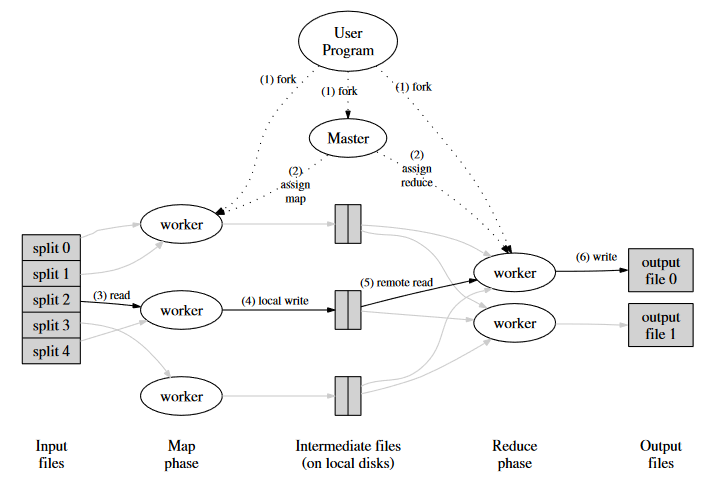
\includegraphics[width=1.0\linewidth]{img/mr-execution}
    \caption[MapReduce execution overview.]{MapReduce execution overview. \cite{dean2008mapreduce}}
    \label{fig:mr-execution}
\end{figure}

The actual architecture of splitting up the work is described in great detail in Dean's paper. We provide a brief overview of it here though. A MapReduce job is initiated by a user library which defines the input data, map task, and reduce task. This job is replicated on many nodes in a cluster. One of the nodes is elected the mater node who assigns $M$ map tasks and $R$ reduce tasks over idle workers. Worker nodes with assigned map tasks transforms their input data with the user defined function and buffers intermediate pairs in memory and sometimes to disk. Worker nodes that were assigned reduce are provided the locations of intermediate data , groups together pairs with the same key, and reduces the values based on the user provided function. The results are these reductions are stored in $R$ files that have to be then managed by the user application. This process is shown in figure \ref{fig:mr-execution}.

The elected master node has several other duties including storing the state of each map and reduce task and also storing the locations of the intermediate pairs produced by the map task.

MapReduce was designed to work in situations of large scale failure. Maps tasks that fail can simple be re-ran. If a worker node goes down, that worker's tasks are assigned to another worker and the computations are re-ran. The only failure condition is in the event of a master failure. In such a case, the entire job will need to be re-submitted to a new master.

As data is distributed, MapReduce attempts to schedule tasks on machines that are close to the data (on GFS) that they wish to access. This is still a hot topic in academia today with ongoing research in scheduling and mapping MapReduce tasks to increase data locality.

Google introduced several refinements on top of the basic MapReduce architecture. These include the ability provide custom partition functions to reduce tasks to control where results are written, ordering guarantees of intermediate keys within a given partition, an intermediate combiner function to combine repetitive date before reduction, auxiliary files as side-effects from tasks, black listing of bad data, local execution for debugging purposes, status information of HTTP, and counters for performance metrics.

Google successfully uses MapReduce at Google for many different purposes including machine learning, clustering, data mining and extraction, web page mining, large-scale graph computations, and more.

\subsubsection{Hadoop}

\subsubsection{Twister}
Twister, described by Ekanayake et al.\cite{ekanayake2010twister}, provides extensions and improvements on top of the MapReduce programming model that open up distributed computing to a wider class of problems.


\subsubsection{Apache Spark}

\subsection{Dryad}
Dryad is a distributed execution engine developed at Microsoft Research by Isard et al. and described in their 2007 paper \textit{Dryad: Distributed Data-Parallel Programs from Sequential Building Blocks}\cite{isard2007dryad}. 

Dryad is described as a ``general-purpose distributed execution engine for coarse-grain data-parallel applications''.

Distributed computations in Dryad are modeled using a directed acyclic graph (DAG) data structure where each node in the graph represents a computation and edges represent data transport (files, TCP, etc).


\subsection{GraphX}



\subsection{Shark}

\subsection{Pregel}
Pregal was designed at Google and is described in the 2010 paper \textit{Pregel: A System for Large-Scale Graph Processing}\cite{malewicz_pregel:_2010} by Malewicz et al.

Pregel was designed as a computational model to compute results on large graph data structures (trillions of edges) using a vertex centered approach where vertices can send and receive messages to other vertices and modify state based on contents of incoming and outgoing messages. 

\subsection{Storm}

\subsection{Tez}

\subsection{PowerGraph}

\subsection{MapReduce/Hadoop and Other Related Technologies}
In this section, we briefly look at several higher level abstractions and technologies that work directly with distributed computation frameworks. As this is not the main focus of this review, we only provide brief descriptions of these technologies. However, we did want to include them for completeness.

SawZall\cite{pike2005interpreting} was created at Google by Rob Pike and others as a procedural language that automates the creation of MapReduce tasks over regularly structured but distributed data sets. 

Pig\cite{olston2008pig} is an Apache project that uses a custom language \textit{Pig Latin} which mixes the declarative style of SQL with the procedural style of map-reduce. The resulting language makes it easy to develop MapReduce jobs and run ad-hoc queries. Pig runs on top of the MapReduce clone, Hadoop.

Hive\cite{thusoo2009hive} is an Apache project for warehousing huge amounts of data on HDFS. Hive provides an SQL like language called \textit{HiveQL} that converts queries into MapReduce, Apache Tez, or Apache Spark jobs. Hive has built-in support for operating on compressed data.

Chukwa\cite{rabkin2010chukwa} is a system for collecting distributed log files stored on HDFS and processing that data using MapReduce.

Mahout\cite{owen2012mahout} is a machine learning framework capable of collective filtering, categorization, clustering, and parallel frequent pattern mining using a distributed cluster and producing MapReduce jobs.

Yarn\cite{vavilapalli2013apache}


\section{Conclusion}

\bibliography{litreview}
\bibliographystyle{plain}

\end{document}
